\documentclass[a4paper,12pt,oneside]{article}

\usepackage{graphicx}
\usepackage{verbatim}
\usepackage{amsmath}
\usepackage[utf8]{inputenc}
\usepackage[colorlinks,bookmarks=false,linkcolor=blue,urlcolor=blue]{hyperref}
\usepackage{booktabs}
\usepackage{subfig}
\usepackage{amssymb}

\paperheight=297mm
\paperwidth=210mm

\setlength{\textheight}{235mm}
\setlength{\topmargin}{-1.2cm}
%\setlength{\footskip}{5mm}
\setlength{\textwidth}{15cm}
\setlength{\oddsidemargin}{0.56cm}
\setlength{\evensidemargin}{0.56cm}

\pagestyle{plain}
\setcounter{secnumdepth}{2}


\newcommand{\mail}[1]{{\href{mailto:#1}{#1}}}
\newcommand{\ftplink}[1]{{\href{ftp://#1}{#1}}}


\begin{document}

\title{Chaos Déterministe}
\author{Laurent Rohrbasser \& Tim Tuuva}

\maketitle
\tableofcontents
\baselineskip=16pt
\parindent=15pt
\parskip=5pt

% \begin{abstract}
% %Résumé de l'expérience, on fait des tps sur le chaos, rappeler vite fait 
% %dire le but de ces manips, qu'est ce qu'on veut?
% \end{abstract}

\newpage

\section{Introduction}
Si on prend deux bâtons et qu'on fixe le bout d'un baton sur l'autre par un axe, et que cet autre bâton est maintenu par un autre axe, on obtient un pendule double, un objet remarquable à la fois pour sa simplicité et son comportement beaucoup moins simple. Poser une balle de ping-pong sur une surface qui vibre, laisser évoluer 3 corps ou plus, massique ou chargé, mettre un aimant dans un champ magnétique oscillant, exiter un ressort attaché à une masse, etc... en fait, dans un grand nombre d'expériences relativement faciles à imaginer, il est possible d'obtenir un comportement relativement complexe à décrire. Cette complexité s'exprimme entre autre par un rapide divergence de la même expérience reproduite avec des conditions initiales similaires et un comportement aperiodique, très difficile à prédire.

Il sera étudié ici deux expériences dont il est possible de facilement prendre des mesures, à savoir un pendule inversé dont l'angle de repos est modifié au cours du temps ainsi qu'un dispositif laissant libre l'orientation d'un aimant qui est plongé dans un champ magnétique qui varie au cours du temps.

% Il existe dans de nombreux dispositifs simples ayant des comportements relativement complexes rendent assez difficile une prédiction même à court terme de l'évolution du dispositif en question, même avec en main les équations décrivant complètement les équations du système : une variation infinitesimale sur un paramètre cause
% En fait il se trouve que ce sont exactement ces équations qui sont responsable du comportement complexe du dispositif.

\section{Quelques notions}
\label{Quelques notions}

Un système physique en mécanique classique peut être décrit par un certain nombre de variables, comme par exemple la position de tous points libres de se déplacer les uns par rapport aux autres, l'angle de chaque bras articulés, ainsi que les dérivées de chacunes de ces variables. Ainsi, on peut entièrement décrire un système avec toutes les valeurs qu'ont ces paramètres, il est alors assez naturel d'introduire un espace de dimension le nombre de degrés de libertés du système décrit (fois deux à cause des dérivées) dans lequel le système est représenté en un temps donné par un point.

Cet espace est appelé \textbf{espace de phase}. Les positions que peut prendre le système sont données par $2n$ valeurs $\{q_i,\dot{q_i}\}$. En fait on peut prendre des fonctions plus compliquées que la simple dérivée temporelle de $p_i$ par rapport au temps (cf mécanique analytique). $\dot{q_i}$ sera aussi appelé $p_i$, mais dans la mesure où ces deux valeurs coincident, on ne fera pas de distinctions ici.
Ainsi en ajoutant un axe de temps à l'espace de phase, on peut ajouter pour chaque valeurs de t la valeur $\{q_i(t),\dot{q_i}(t)\}$ correspondante, et donc observer la trajectoire qu'à suivi le système dans l'espace de phase en projetant sur n'importe quel plan $t=cst$.

Les systèmes observés dans ce cadre sont décrit par des \textbf{potentiels oscillant} sur une période $\tau$ constante dans chaque expérience. Une idée est alors d'enrouler l'axe du temps sur lui même de telle sorte qu'un tour corresponde à $\tau$. Ainsi on peut observer par quels points de l'espace de phase passe le système à chaque fois que le potentiel dans lequel il se trouve reprend la même allure. La tranche de la trajectoire donnée par tous les points tels que $t=n\tau$ avec $n\in \mathbb{N}$ s'appelle la \textbf{section de Poincaré}. Cette section permet de décrire qualitativement le comportement du système selon le choix de paramètres de l'expérience (valeur de la période $\tau$, amplitude de la variation du potentiel etc...) : dans les cas les plus simples, on peut voir un nombre fini de points, ce qui correspond au fait que le pendule a une période de $k\tau$ avec $k$ valant le nombre de points observé sur la section. Mais il arrive parfois qu'il y ait un grand nombre de points, le tout sur une figure formant des fractales (cf simulations numériques). Le nombre de points défni en fait le nombre d'orbites sur lesquels le système oscille.

Pour ranger les différentes zones par nombre d'orbites, on peut projeter les points $\{q_i,\dot {q_i}\}$ sur une droite et compter les points (en supposant les superpositions rares). En itérant sur un paramètre de l'expérience, on peut mettre chaque nuage de points obtenu les uns à côté, et voir dans quelles régions le nombre d'orbites est fini, et dans quelles régions il explose. La figure obtenue s'appelle un \textbf{diagramme de bifurcation}.



\section{Dispositif}
%Description du dispositif expérimental
%Tim's duty
\subsection{Pendule inversé}

\subsubsection{Matériels}
%Oui c'est du copier coller je vais voir si je change ca
\begin{itemize}
  \item[--] Générateur de tension.
  \item[--] Générateur LD Series (A+D Products Bienne CH, EPFL TP Physique 466).
  \item[--] Pendule inversé (EPFL TP Physique 41).
  \item[--] Boitier ’Pendule chaotique’.
  \item[--] Boitier SensorCassy (Leybold Didactic Gmbh).
  \item[--] Voltmètre.
\end{itemize}

% \subsubsection{Schéma}

% \begin{figure}[h!]
%   \begin{center}
%   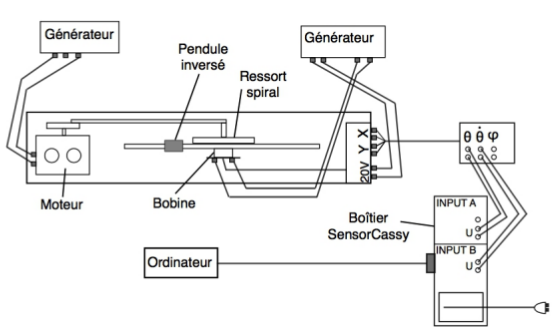
\includegraphics[width=0.5\linewidth,angle=0]{./figures/pendule_inverse.png}
%   \caption{Schéma du dispositif du pendule inversé pour le TP sur le chaos déterministe.} \label{fig:pendule1}
%   \end{center}
% \end{figure}
\begin{figure}[h!]
  \begin{center}
  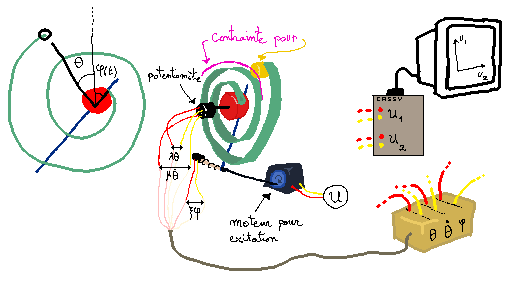
\includegraphics[width=1\linewidth,angle=0]{./figures/pendule.png}
  \caption{Schéma du dispositif du pendule inversé pour le TP sur le chaos déterministe.} \label{fig:pendule1}
  \end{center}
\end{figure}

\subsubsection{Description}

%TODO PEAUFINER
Le pendule inversé est muni d'un potentiomètre, alimenté par un premier générateur, dont la position angulaire correspond à $\theta$. Le dispositif permet aussi de mesurer la vitesse angulaire $\dot{theta}$ par une différence de potentiel. Le dispositif est relié à un amplificateur.
Un boitier SensorCassy mesure le potentiel amplifié, le digitalise et passe les valeurs lues à un ordinateur, ce qui permet de relever les différentes valeurs de $\theta$ et $\dot{\theta}$ au cours du temps, ce qui permet de tracer les différetes positions prises par le pendule dans l'espace de phase.
Un moteur alimenté par un deuxième générateur, peut provoquer une perturbation sur l'axe du ressort : le moteur permet d'agiter la position d'équilibre du pendule, ce qui a pour effet d'exiter la masse et donc de le mettre en mouvement. Un autre appareil est mis à disposition pour mesurer la position du moteur d'exitation.
Il est aussi possible d'utiliser un frein electromagnétique pour réaliser une autre forme de perturbation.

\subsubsection{Procédure}

L'expérience consiste à observer le comportement du pendule pour différents :
\begin{itemize}
  \item[-] fréquence d'exitation
  \item[-] frottement
  \item[-] position équilibre du pendule (réalisée par accident)
\end{itemize}

Les observations se font à travers la construction de diagramme de phase et de courbes d'évolution temporelle de chacunes des variables décrivant le pendule ($\theta$ et $\dot{\theta}$), l'idée étant de décrire qualitativement la réaction du comportement du pendule aux variations de chaque paramètres.


Le moteur est alimenté avec $U_{alimentation}=2\sim10$ [V].
La sonde du pendule est alimentée avec $U_{alimentation}=10\sim20$ [V]. Le choix de $U_{alimentation}$ sert notemment à observer soit de grande oscillations, soit de petites oscillations : un grand $U$ peut impliquer des saturations dans les appareils d'aquisitions pour de grandes variations de $\theta$.
\subsection{Moteur dipolaire}

\subsubsection{Materiels}
\begin{itemize}
  \item[--] Générateur de fonctions: Wavetek, IPE 241-07/03.
  \item[--] Générateur d’impulsions: EPFL, IPE 242 - 07/03.
  \item[--] Oscilloscope: Hewlett Packard, HP 54600A.
  \item[--] Sonde de Hall : Bell 620 Gaussmeter, IPE 240 - 07/03.
  \item[--] Amplificateur C.C. : EPFL.
  \item[--] Moteur bipolaire : EPFL.
\end{itemize}

% \subsubsection{Schéma}
% \begin{figure}[h!]
%   \begin{center}
%   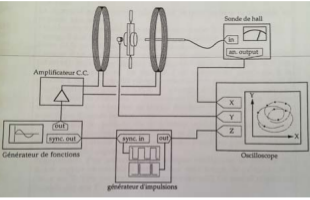
\includegraphics[width=0.6\linewidth,angle=0]{./figures/moteur1.png}
%   \caption{} \label{fig:}
%   \end{center}
% \end{figure}
% \subsubsection{Schéma}
\begin{figure}[h!]
  \begin{center}
  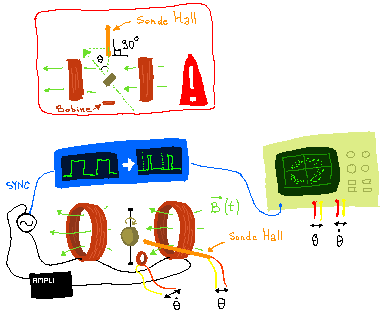
\includegraphics[width=1\linewidth,angle=0]{./figures/pendule_2.png}
  \caption{} \label{fig:pendule_2}
  \end{center}
\end{figure}


\subsubsection{Description}
\label{description}

Un générateur de fonction branché à un amplificateur C.C. permet d'envoier un signal triangulaire dans une paire de bobines comme illustré dans le schémas \ref{fig:pendule_2}. Ce courant permet de créer un champ magnétique à peu près linéaire dans le volume entre les deux bobines, ce qui a pour effet d'exiter l'aimant de Helmotz ayant la liberté de rotater autour d'un axe (cf fig \ref{fig:pendule_2}).

Une sonde Hall est installée dans la direction orthogonale au champ généré par les bobines, et qui se trouve sur le plan dans lequel rotate l'aimant. Mesurant la composante du champ magnétique orthogonale à celui généré par les bobines, cette sonde mesure le champ généré par l'aimant de Helmotz dans une direction, et ainsi elle permet la mesure de l'angle de l'aimant par rapport à l'axe des bobines.

Une bobine disposée comme la sonde Hall permet de mesurer les variations du champ magnétique par induction de courant, ainsi il est possible de mesurer $\dot{\theta}$.

Avec toutes ces mesures, il est alors facile d'afficher l'état du pendule dans son espace de phase : il suffit de brancher la sonde Hall à l'entrée X et la bobine à l'entrée Y, en plottant X(Y), on a immédiatement à l'écran de l'oscilloscope la position du pendule dans son espace de phase.

Il est possible d'obtenir une section de Poincaré en utilisant le trigger du générateur (explications données dans la section \ref{Quelques notions}), en intégrant dans le temps tous les passages du pendule dans le plan $t=n\tau$, $n\in \mathbb{N}$, où $\tau=1/\nu$ avec $\nu$ la fréquence d'exitation.

\subsubsection{Procédure}

Il est ici observé les différents comportement du pendule magnétique pour différentes valeurs du champ magnétique permanant appliqué et différentes valeurs de fréquence d'exication. Il est introduit un paramètre $F=f/\omega^2$ avec $\omega$ la pulsation d'exitation et $f=\frac{\mu B}{I}$, $I$ étant le moment d'inertie de l'aimant, $B$ le champ magnétique qui lui est appliqué, $\mu$ le moment magnétique de l'aimant.

Le but est d'observer le comportement de l'aimant selon ce paramètre $F$, or sachant que f est une fonction du courant circulant dans les bobines, on peut garder $\omega$ constant et varier ce courant pour changer $B$ et réaliser un diagramme de bifurcation. Le diagramme sera la projection de la section de Poincaré sur l'axe $\dot{\theta}$ en fonction de $F$.

Il est aussi réalisé quelques sections de Poincaré.


% le moteur dipolaire a une fréquence propre d'oscillation $f\approx1.75$ [Hz], forcant sa redirection momentanément. 

\section{Résultats}

\subsection{Pendule inversé}

Une première observation que l'on peut faire est la sensibilité aux conditions.
Lorsqu'on s'intéresse à l'évolution de chaque variables du système au cours du temps, dans les cas non chaotiques, on constate que si la distance des deux expériences est faible dans l'espace de phase, l'évolution sera à peu près la même pour les deux systèmes pour des temps relativement longs. Il n'en est pas de même pour les systèmes chaotique : comme il peut être constaté dans le graphe \ref{fig:comparaison}, deux systèmes très proches dans l'espace de phase divergent très rapidement. Le système étant exité, il a été rajouté le graphe \ref{fig:comparaison2} qui montre que même les moteurs avaient des positions très similaires, et donc qu'il s'agit bien d'une divergence dûe au comportement du système.

 

\begin{figure}[h!]
  \begin{center}
  \includegraphics[width=1.0\linewidth,angle=0]{./figures/comparaison.pdf}
  \caption{Comparaison du mouvement du pendule selon différente conditions initiales. Il est apparent que ce mouvemnt est chaotique. %Réalisé avec $\omega \approx XXX$
  } \label{fig:comparaison}
  \end{center}
\end{figure}

L'autre fait intéressant dans l'observation de ce second graphe est l'apparente convergence sur une orbite : bien que toutes les expériences soient très différentes à une échelle microscopique d'un point de vue temporel, on constate que les parcours sur l'espace de phase est lui très similaire dans tous les cas.

\begin{figure}[h!]
  \begin{center}
  \includegraphics[width=1.0\linewidth,angle=0]{./figures/comparaison2.pdf}
  \caption{Comparaison du mouvement du pendule selon différente conditions initiales. Il est apparent que ce mouvemnt est chaotique. On ajoute ici la position du moteur au cours du temps pour s'assurer qu'il s'agit bien de trois fois la même expérience} \label{fig:comparaison2}
  \end{center}
\end{figure}

Étant donné que le système passe par de nombreux points éloignés, mais reste en orbite autour d'une figure, il devient alors assez immédiat de vouloir tester des conditions initiales très différentes pour voir si le pendule tend vers ces mêmes orbites. La figure \ref{fig:1_3_U_5_01_lab} illustre le résultat d'un telle expérience : en effet dans la plus part des cas, l'orbite converge vers quelque chose. Cette chose est ce qu'on appelle un \textbf{attracteur étrange}.

Une chose intéressante est que pour les mêmes paramètres pour l'expérience, choisir une condition initiale pour le pendule lui fournissant une plus grande énergie a pour conséquence que l'orbite change, comme on peut le voir sur la courbe noire dans la figure \ref{fig:1_3_U_5_01_lab}. En plus de cela, le comportement chaotique avait disparu : l'orbite était plutôt régulière.

\begin{figure}[h!]
  \begin{center}
  \includegraphics[width=1.0\linewidth,angle=0]{./figures/1_3_U_5_01_lab.pdf}
  \caption{Illustration de la différence de mouvement selon différentes conditions initiales. Avec une plus grande énergie initiale l'aspect chaotique disparait.} \label{fig:1_3_U_5_01_lab}
  \end{center}
\end{figure}

\begin{figure}[h!]
  \begin{center}
  \includegraphics[width=1.0\linewidth,angle=0]{./figures/potentiel.pdf}
  \caption{allure du potentiel :$V(\theta,t)=\frac{1}{2}k(\theta-a sin(\omega t))^2-\frac{1}{2} m g cos(\theta)$} \label{fig:potentiel}
  \end{center}
\end{figure}



Après avoir effectué un balayage sur une large gamme de fréquence d'exitation, il a pu être constaté que l'obtention du chaos était favorisé par des fréquences de l'ordre de la fréquence propre du pendule, le tout combiné avec un frottement.

En effet pour les exitations trop lentes, le pendule ne fait que passe d'un point d'équilibre à l'autre avec peut d'oscillations, souvent le pendule se trouve dans un des puits de potentiel à droite ou à gauche, et oscille dans les déplacements du puits, sans passer dans le puits situé de l'autre côté (cf figure \ref{fig:potentiel}). Et si la fréquence est trop élevée, le pendule n'accumule pas d'énergie et ne fait que de très faibles oscillations autours de son point d'équilibre.

L'effet du frottement est montré dans la figure \ref{fig:1_2_U_4_97_theta__FREIN_PAS_FREIN_lab} : il a pu être observé a plusieur reprise que l'ajout de frottement dans un pendule dans un régime non chaotique a contribué à un changement de régime aboutissant à un comportement chaotique. Ici le pendule se met à passer d'un creux de potentiel à l'autre de façon assez imprédictible. On observe des traces de l'asymétrie du pendule par une préférence d'un des puits sur l'autre.

\begin{figure}[h!]
  \begin{center}
  \includegraphics[width=0.8\linewidth,angle=0]{./figures/1_2_U_4_97_theta__FREIN_PAS_FREIN_lab.pdf}
  \caption{Passage d'un mode périodique à un mode chaotique par application d'un frein électromagnétique} \label{fig:1_2_U_4_97_theta__FREIN_PAS_FREIN_lab}
  \end{center}
\end{figure}


Un autre paramètre ayant une certaine importance dans l'obtention du chaos dans cette expérience a été la symétrie du pendule : si le point d'équilibre du pendule n'était pas au plus haut, un des côtés (droite ou gauche) avait un puit de potentiel plus profond. La conséquence de ceci est qu'il devient alors difficile d'observer des oscillations dans lesquelles le pendule reste pendant un moment à droite et pendant un autre à gauche : il n'a tendance à osciller que d'un seul côté (cf graphe \ref{fig:1_2_U_3_44_lab}). 


\begin{figure}[h!]
  \begin{center}
  \includegraphics[width=0.8\linewidth,angle=0]{./figures/1_2_U_3_44_lab.pdf}
  \caption{Le pendule tombe constemment du même côté, il faut le rééquilibrer} \label{fig:1_2_U_3_44_lab}
  \end{center}
\end{figure}





\clearpage










% \clearpage


% \begin{comment}\begin{figure}[h!]
%   \begin{center}
%   \includegraphics[width=1.0\linewidth,angle=0]{./figures/1_1_001_lab.pdf}
%   \caption{Illustration de la difficulté à obtenir une symétrie du pendule inversé tel qu'il y a deux positions d'équilibre.} \label{fig:1_1_001_lab}
%   \end{center}
% \end{figure}

% \begin{figure}[h!]
%   \begin{center}
%   \includegraphics[width=1.0\linewidth,angle=0]{./figures/1_1_008_lab.pdf}
%   \caption{Tentative de rééquilibrage du pendule, la position de repos du pendule est passé de droite à gauche, cependant la présence d'une double position d'équilibre n'est pas encore effective.} \label{fig:1_1_008_lab}
%   \end{center}
% \end{figure}


% \begin{figure}[h!]
%   \begin{center}
%   \includegraphics[width=1.0\linewidth,angle=0]{./figures/1_2_U_10_95_lab.pdf}
%   \caption{Illustration de l'inutilité d'appliquer une fréquence trop élevé au pendule avec $\omega\approx XXX$.} \label{fig:1_2_U_10_95_lab}
%   \end{center}
% \end{figure}

% \begin{figure}[h!]
%   \begin{center}
%   \includegraphics[width=1.0\linewidth,angle=0]{./figures/1_2_U_2_41_lab.pdf}
%   \caption{$\omega \approx$} \label{fig:1_2_U_2_41_lab}
%   \end{center}
% \end{figure}
% \end{comment}

% \begin{figure}[!ht]
%     \subfloat[Équilibre à droite.\label{fig:subfigeqd}]{%
%       \includegraphics[width=0.5\textwidth]{./figures/1_1_001_lab.pdf}
%     }
%     \hfill
%     \subfloat[Équilibre à gauche.\label{fig:subfigeqg}]{%
%       \includegraphics[width=0.5\textwidth]{./figures/1_1_008_lab.pdf}
%     }
%     \caption{Illustration de la difficulté à obtenir une symétrie du pendule inversé tel qu'il y a deux positions d'équilibre.}
%     \label{fig:equilibre}
% \end{figure}

% %La figure~\ref{fig:equilibre} montre la position d'équilibre du pendule inversé dans un diagrame de phase $(\theta,\dot{\theta})$, avant et après une tentative de rééquilibrage. Ce diagramme est réalisé par une oscillation propre du pendule sans perturbation, la figure de gauche correspond à avant la tentative. Dans ce cas la position d'équilibre était à gauche. À droite, le graphe du pendule avec une correction trop prononcé à gauche.

% \begin{figure}[!ht]
%     \subfloat[$\omega \approx XXX$\label{fig:subfigwpetit}]{%
%       \includegraphics[width=0.5\textwidth]{./figures/1_2_U_10_95_lab.pdf}
%     }
%     \hfill
%     \subfloat[$\omega \approx XXX$.\label{fig:subfigwgrand}]{%
%       \includegraphics[width=0.5\textwidth]{./figures/1_2_U_2_41_lab.pdf}
%     }
%     \caption{Illustration de la marges d'action sur le pendule selon la fréquence d'excitation causé par le moteur.}
%     \label{fig:vitesse}
% \end{figure}

% %La figure~\ref{fig:vitesse} montre une comparaison de la vitesse du moteur excitant le pendule inversé. À gauche, la fréquence étant très élevé ($\omega \approx XXX$) alors qu'à droite, le pendule subit une fréquence de perturbation faible ($\omega \approx$).

% \begin{figure}[h!]
%   \begin{center}
%   \includegraphics[width=1.0\linewidth,angle=0]{./figures/1_2_U_3_02_lab.pdf}
%   \caption{Présence d'un attracteur aux abords de la position droite du pendule, $\omega \approx$} \label{fig:1_2_U_3_02_lab}
%   \end{center}
% \end{figure}

% %La figure~\ref{fig:1_2_U_3_02_lab} représente le diagramme de phase du pendule avec une fréquence d'excitation $\omega \approx XXX$.


% %La figure~\ref{fig:1_2_U_3_44_lab} représente l'étude sur la convergence vers un point d'équilibre du pendule. Ce point d0équilibre est sur la gauche selon l'axe de symétrie du pendule.

% \begin{figure}[h!]
%   \begin{center}
%   \includegraphics[width=1.0\linewidth,angle=0]{./figures/1_2_U_4_54_lab.pdf}
%   \caption{Illustration de la convergence vers une position d'équilibre du pendule, malgré une perturbation crée par le moteur, avec $\omega \approx$Illustration de la convergence vers une position d'équilibre du pendule, malgré une perturbation crée par le moteur, avec $\omega \approx$} \label{fig:1_2_U_4_54_lab}
%   \end{center}
% \end{figure}


% %Une étude sur l'impact du frein électromagnétique sur le pendule a permis d'obtenir la figure~\ref{fig:1_2_U_4_97_theta__FREIN_PAS_FREIN_lab}, réalisé avec $\omega \approx XXX$.

% \begin{figure}[h!]
%   \begin{center}
%   \includegraphics[width=1.0\linewidth,angle=0]{./figures/1_2_U_5_63_lab.pdf}
%   \caption{Problème de symétrie} \label{fig:1_2_U_5_63_lab}
%   \end{center}
% \end{figure}







% \clearpage
% \clearpage












%Sur la figure~\ref{fig:comparaison}, le graphe de $\theta(t)$ selon différents conditions initiales, à une fréquence d'excitation $\omega \approx XXX$.
\subsection{Moteur dipolaire}

Après avoir réalisé des sections de Poincaré par des simulations numérique, il a pu être constaté qu'il est beaucoup plus difficile d'obtenir des figures avec beaucoup de détail expérimentalement. Les figures \ref{fig:dipol1T}, \ref{fig:dipol2T} et \ref{fig:chaos} sont des sections de Pointcaré obtenu expérimentalement et la figure \ref{fig:poincare_beauty} présente ce qu'on a pu obtenir numériquement. Les figures \ref{fig:dipol1T} et \ref{fig:dipol2T} montrent un nombre fini est faible d'orbites sur lesquels oscille l'aimant, cependant la figure \ref{fig:chaos} montre une plus grande irrégularité : nous sommes en présence d'un comportement chaotique.






\begin{figure}[h!]
  \begin{center}
  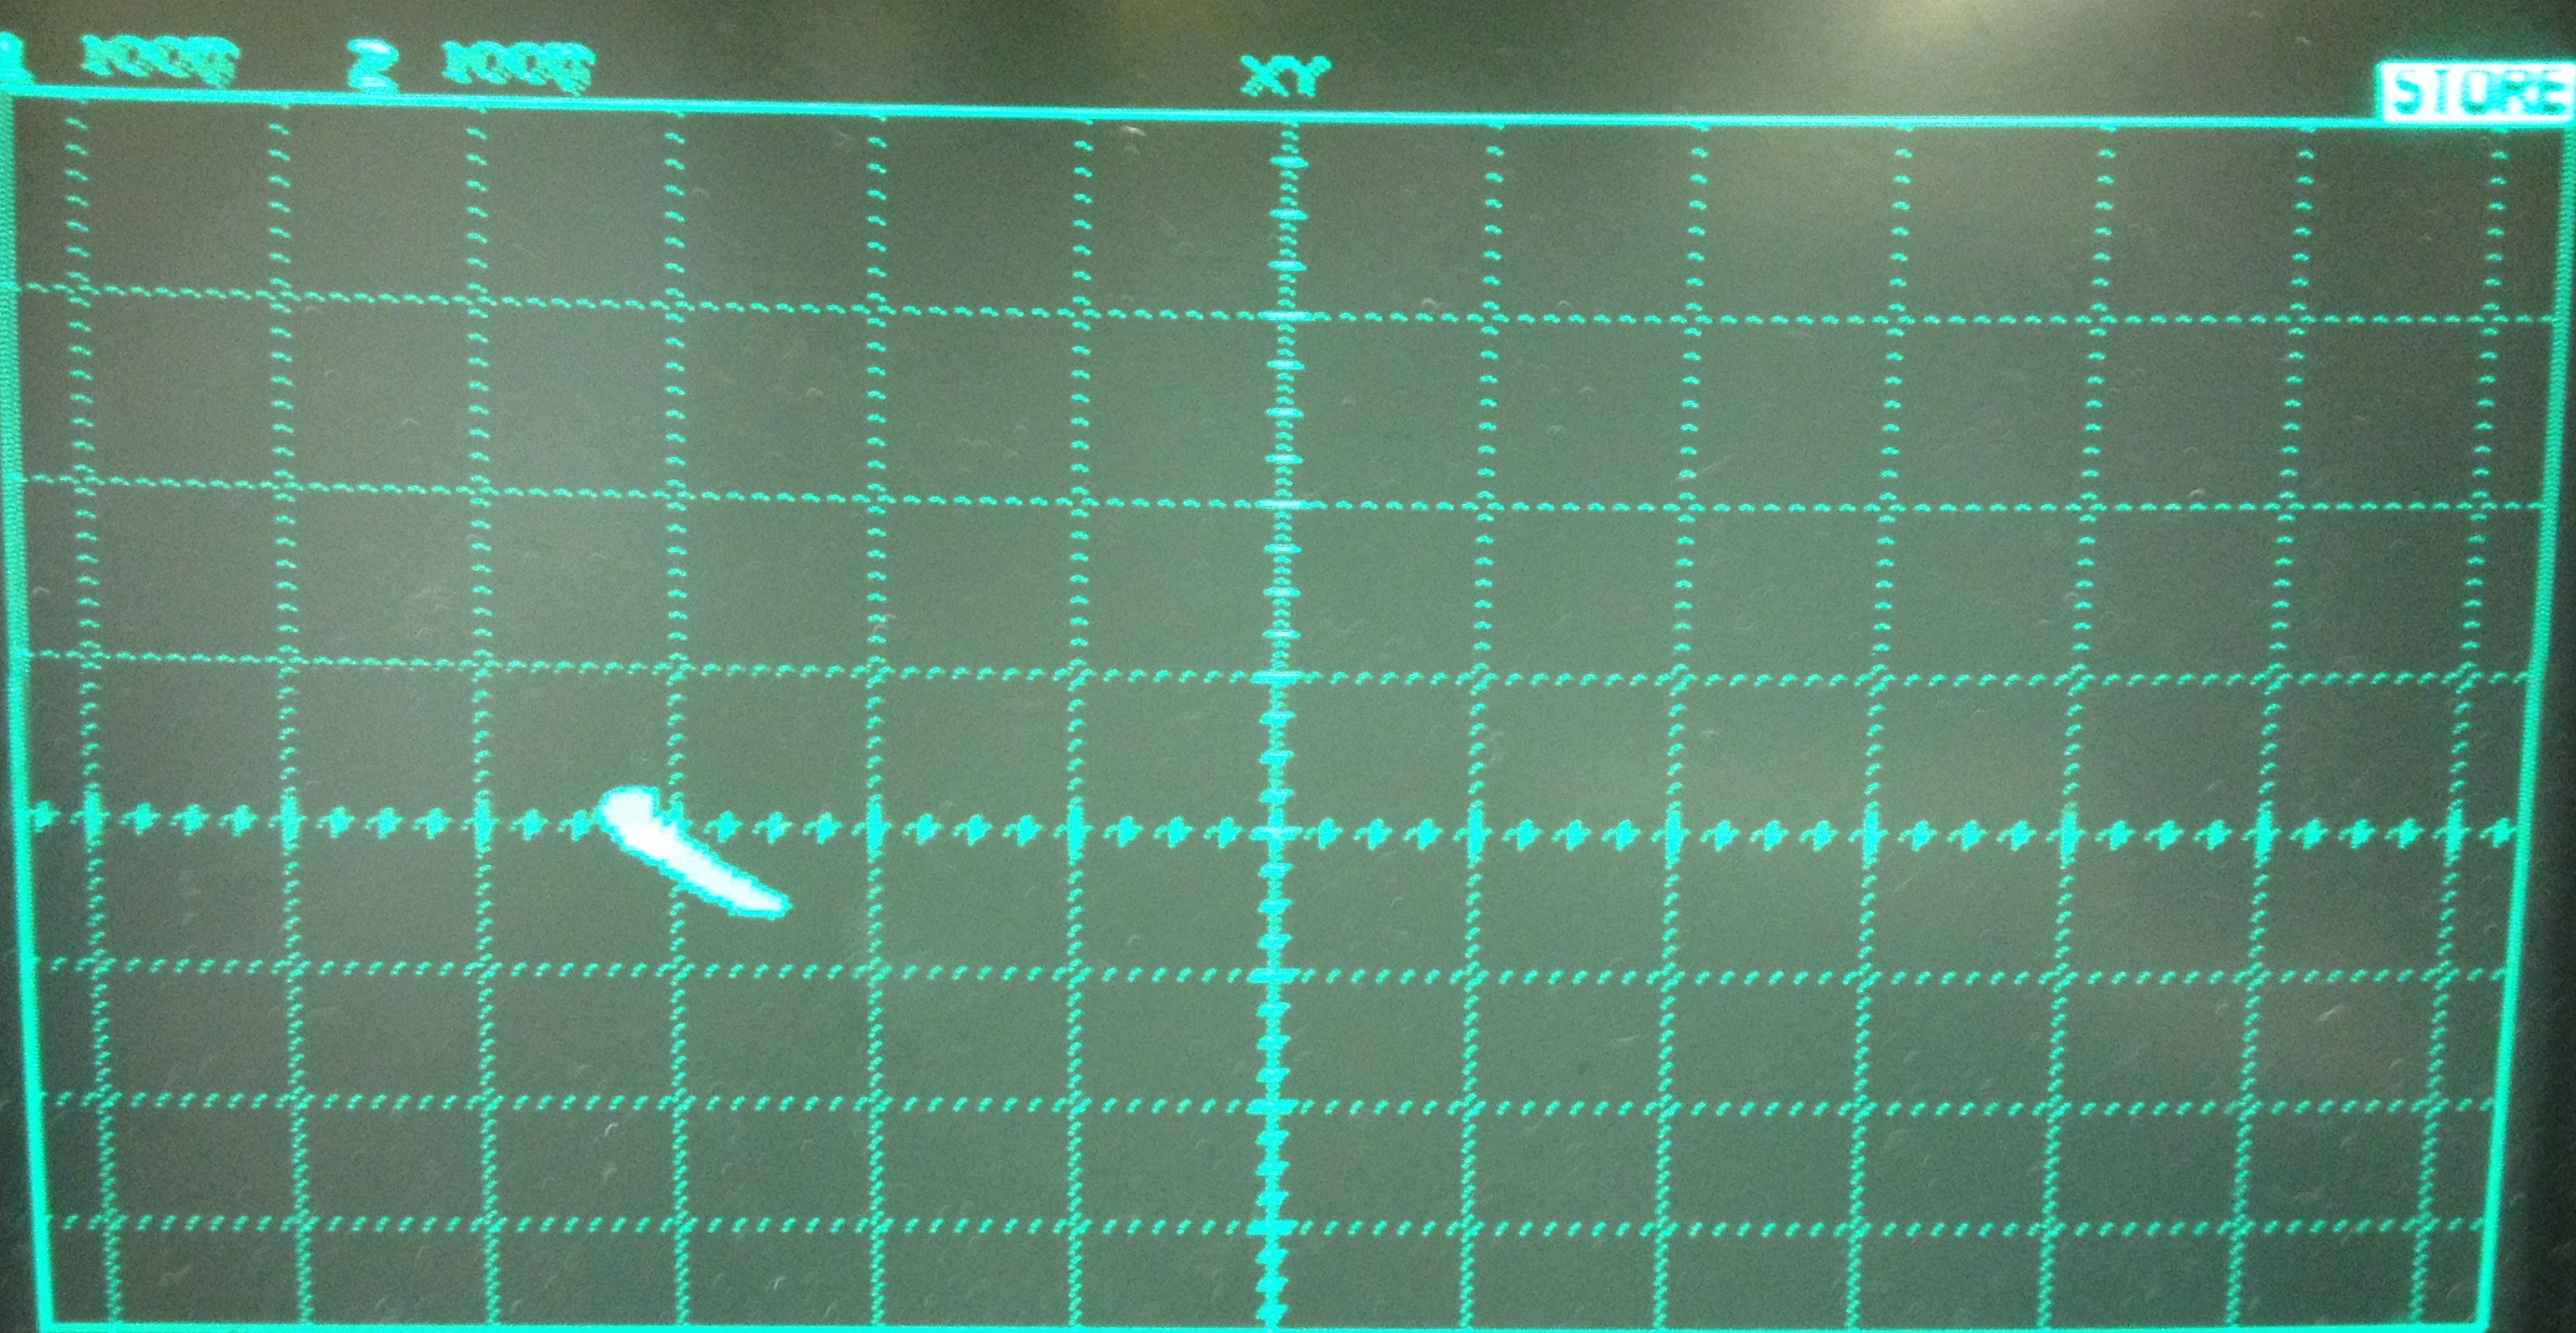
\includegraphics[width=.5\linewidth,angle=0]{./figures/1T_1_18Hz.png}
  \caption{Section de poincaré du diagramme $(\theta,\dot{\theta})$ du moteur dipolaire. Avec une fréquence d'excitation $f=1.18$ [Hz] le pendule a un mouvement une fois périodique.} \label{fig:dipol1T}
  \end{center}
\end{figure}

\begin{figure}[h!]
  \begin{center}
  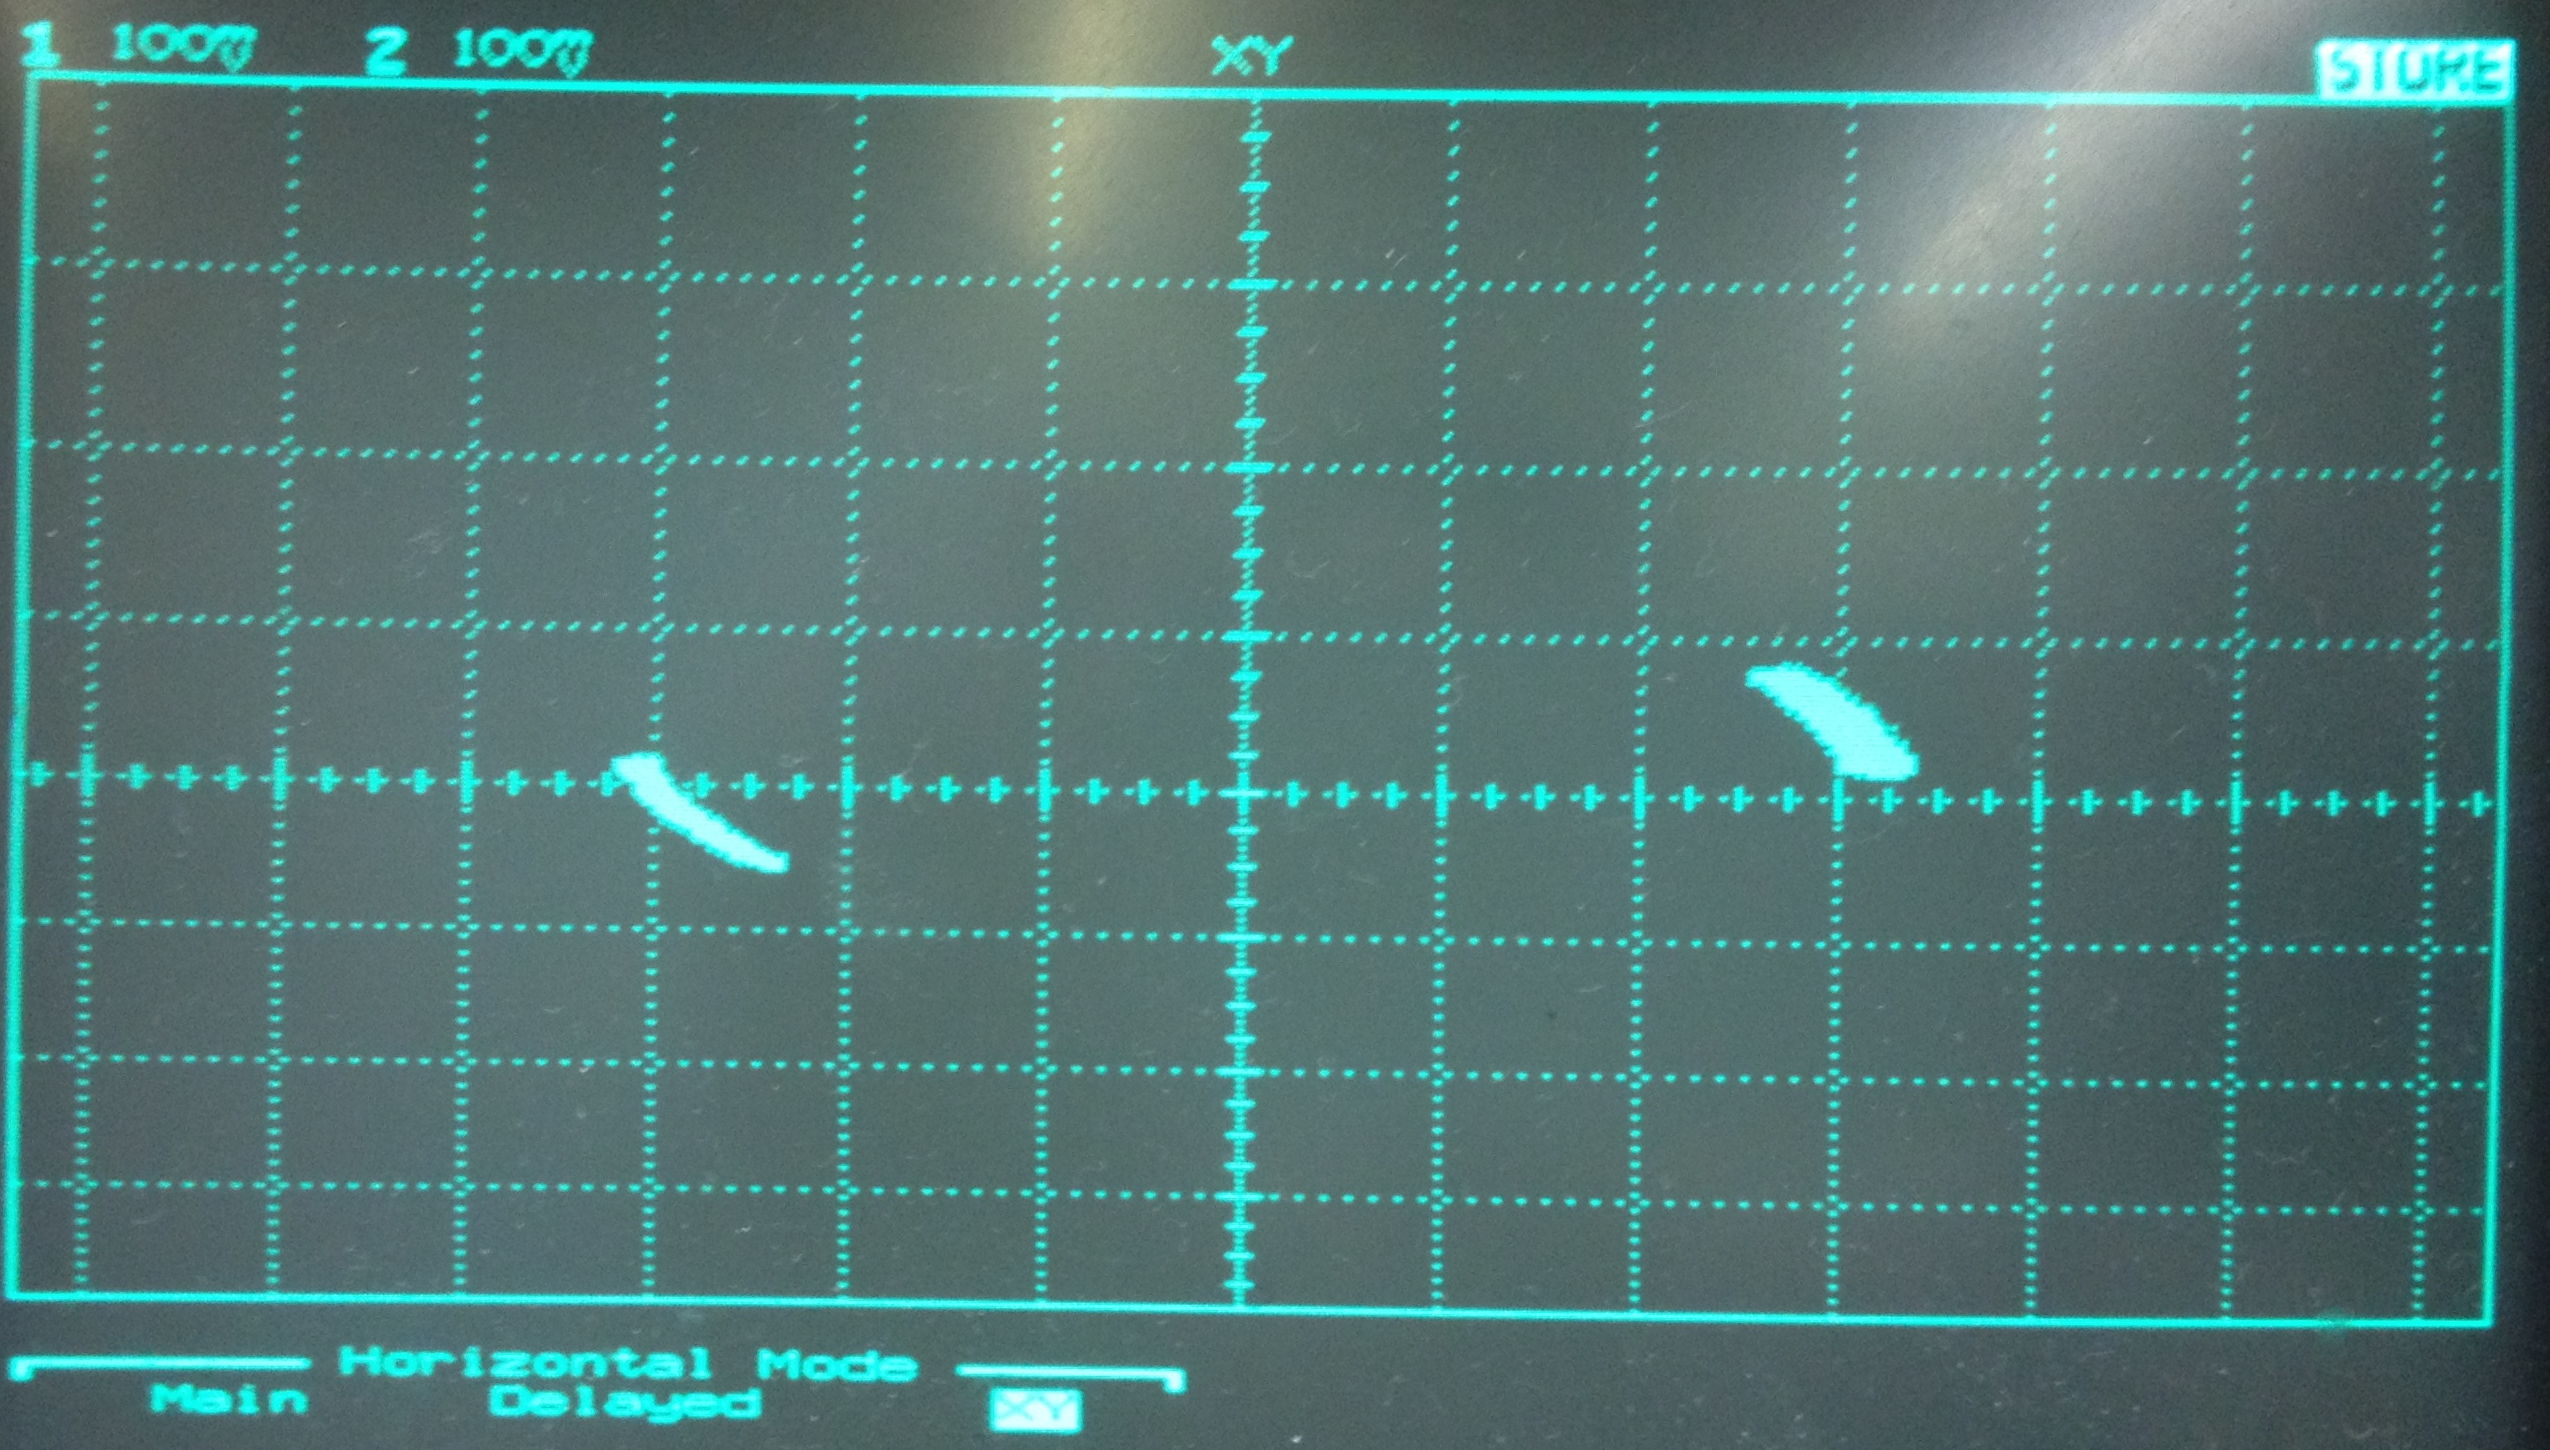
\includegraphics[width=0.5\linewidth,angle=0]{./figures/2T_0_48Hz.png}
  \caption{Section de poincaré du diagramme $(\theta,\dot{\theta})$ du moteur dipolaire. Avec une fréquence d'excitation $f=0.48$ [Hz] le pendule a un mouvement deux fois périodique.} \label{fig:dipol2T}
  \end{center}
\end{figure}

\begin{figure}[h!]
  \begin{center}
  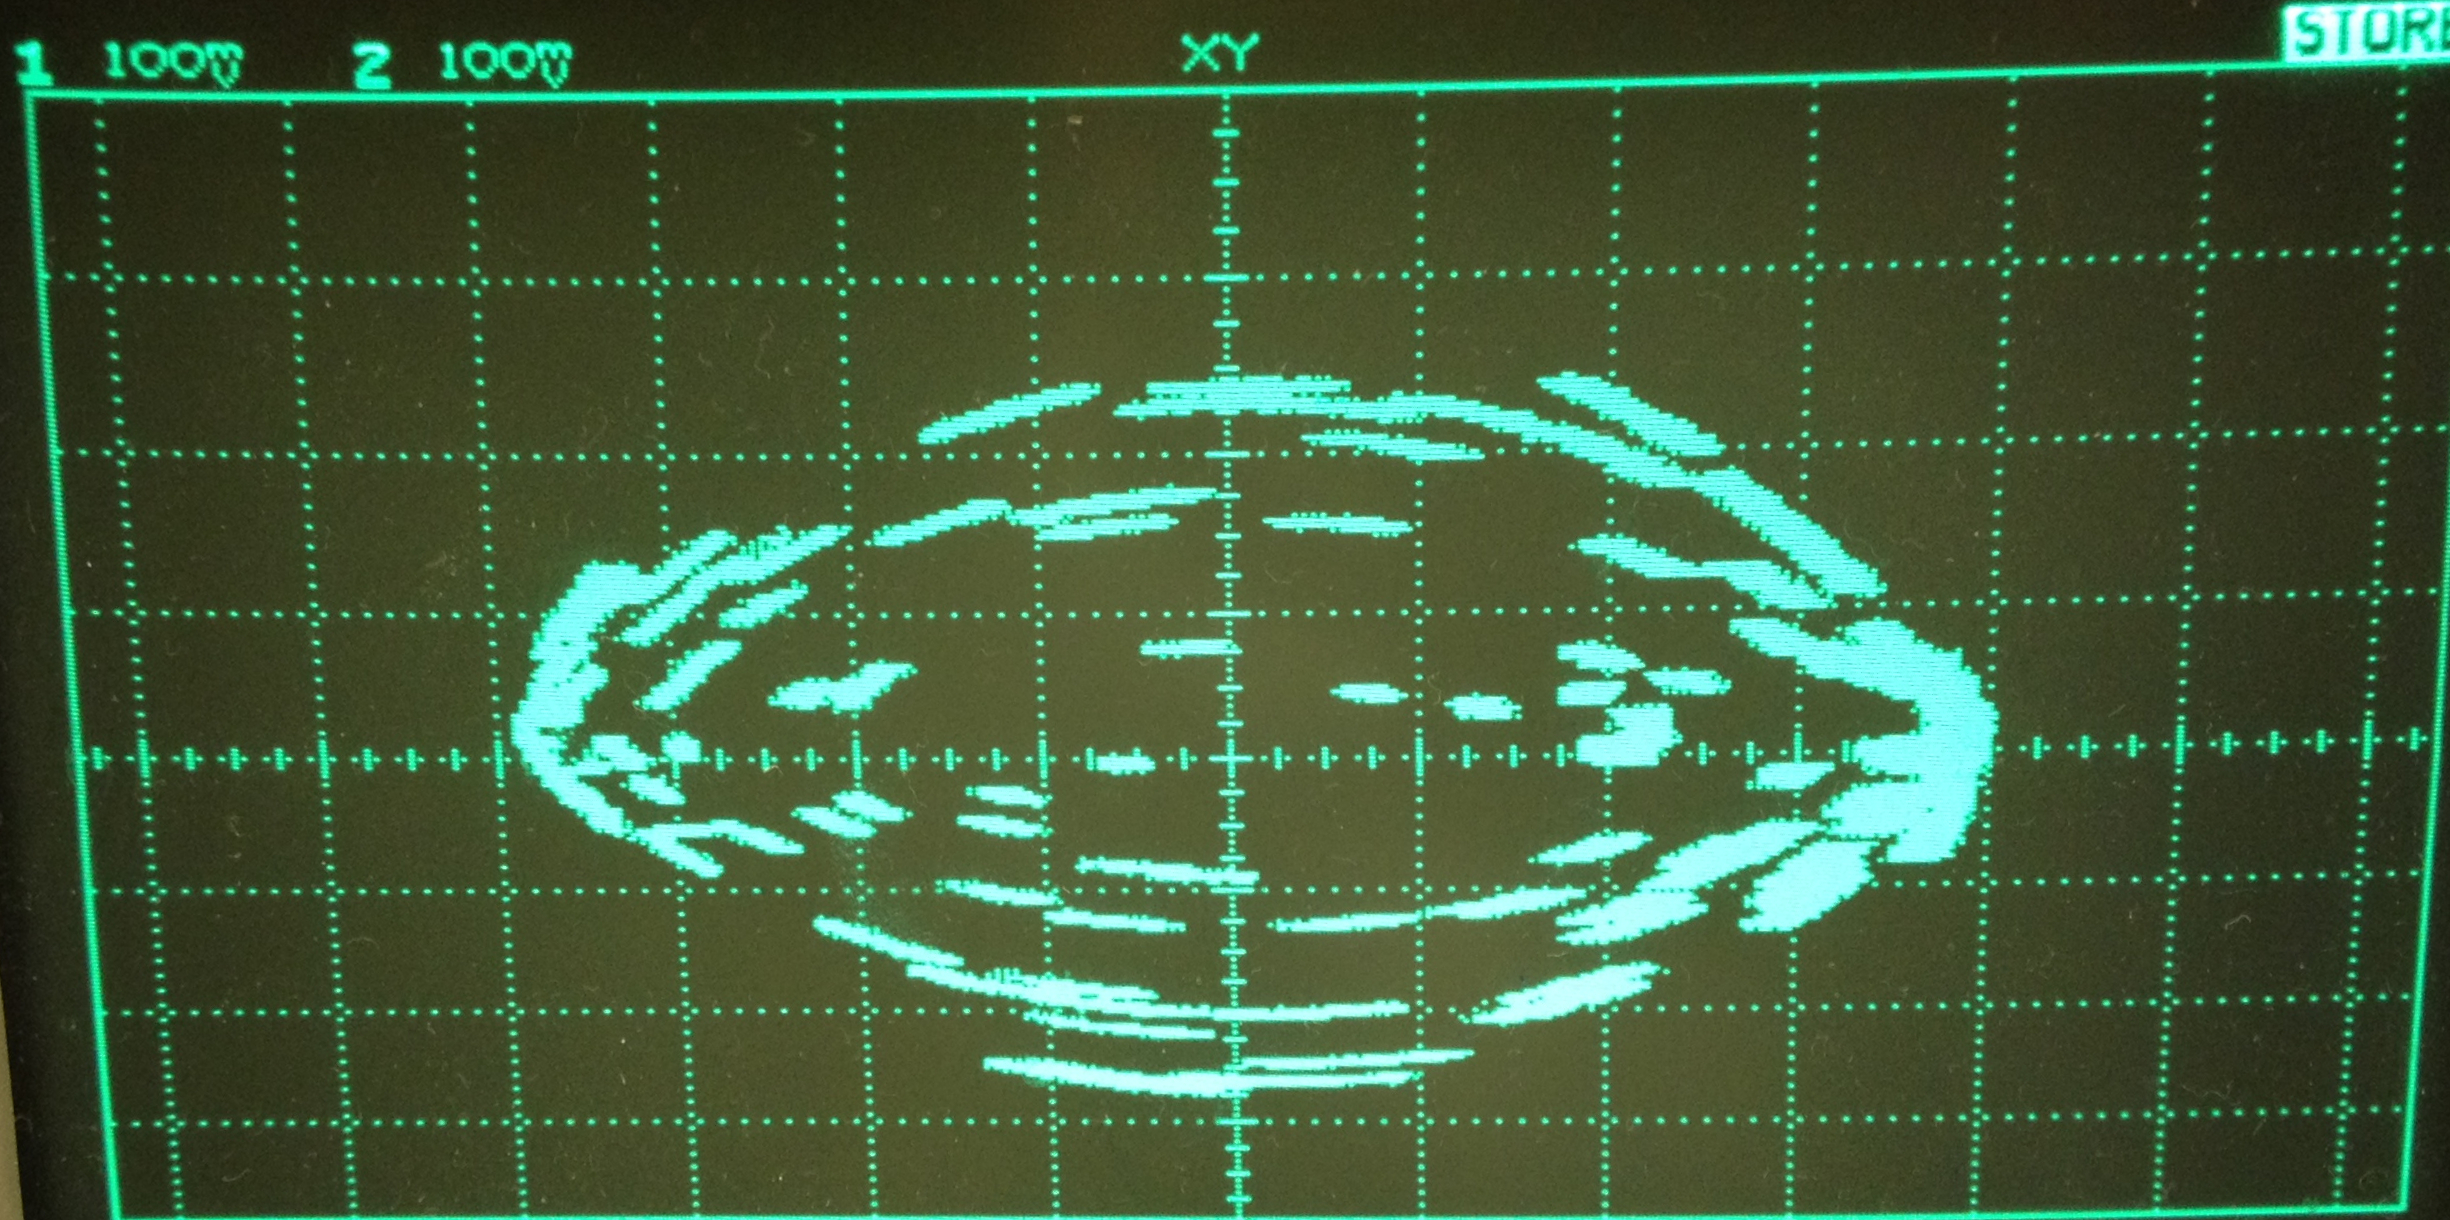
\includegraphics[width=0.5\linewidth,angle=0]{./figures/chao_1_22Hz_v2.png}
  \caption{Section de poincaré du diagramme $(\theta,\dot{\theta})$ du moteur dipolaire. Avec une fréquence d'excitation $f=1.22$ [Hz] le pendule a un mouvement chaotique.} \label{fig:chaos}
  \end{center}
\end{figure}








% \begin{figure}[!ht]
%     \subfloat[$\omega=2\pi1.18$ [Hz], mouvement une fois périodique.\label{fig:dipol1T}]{
%       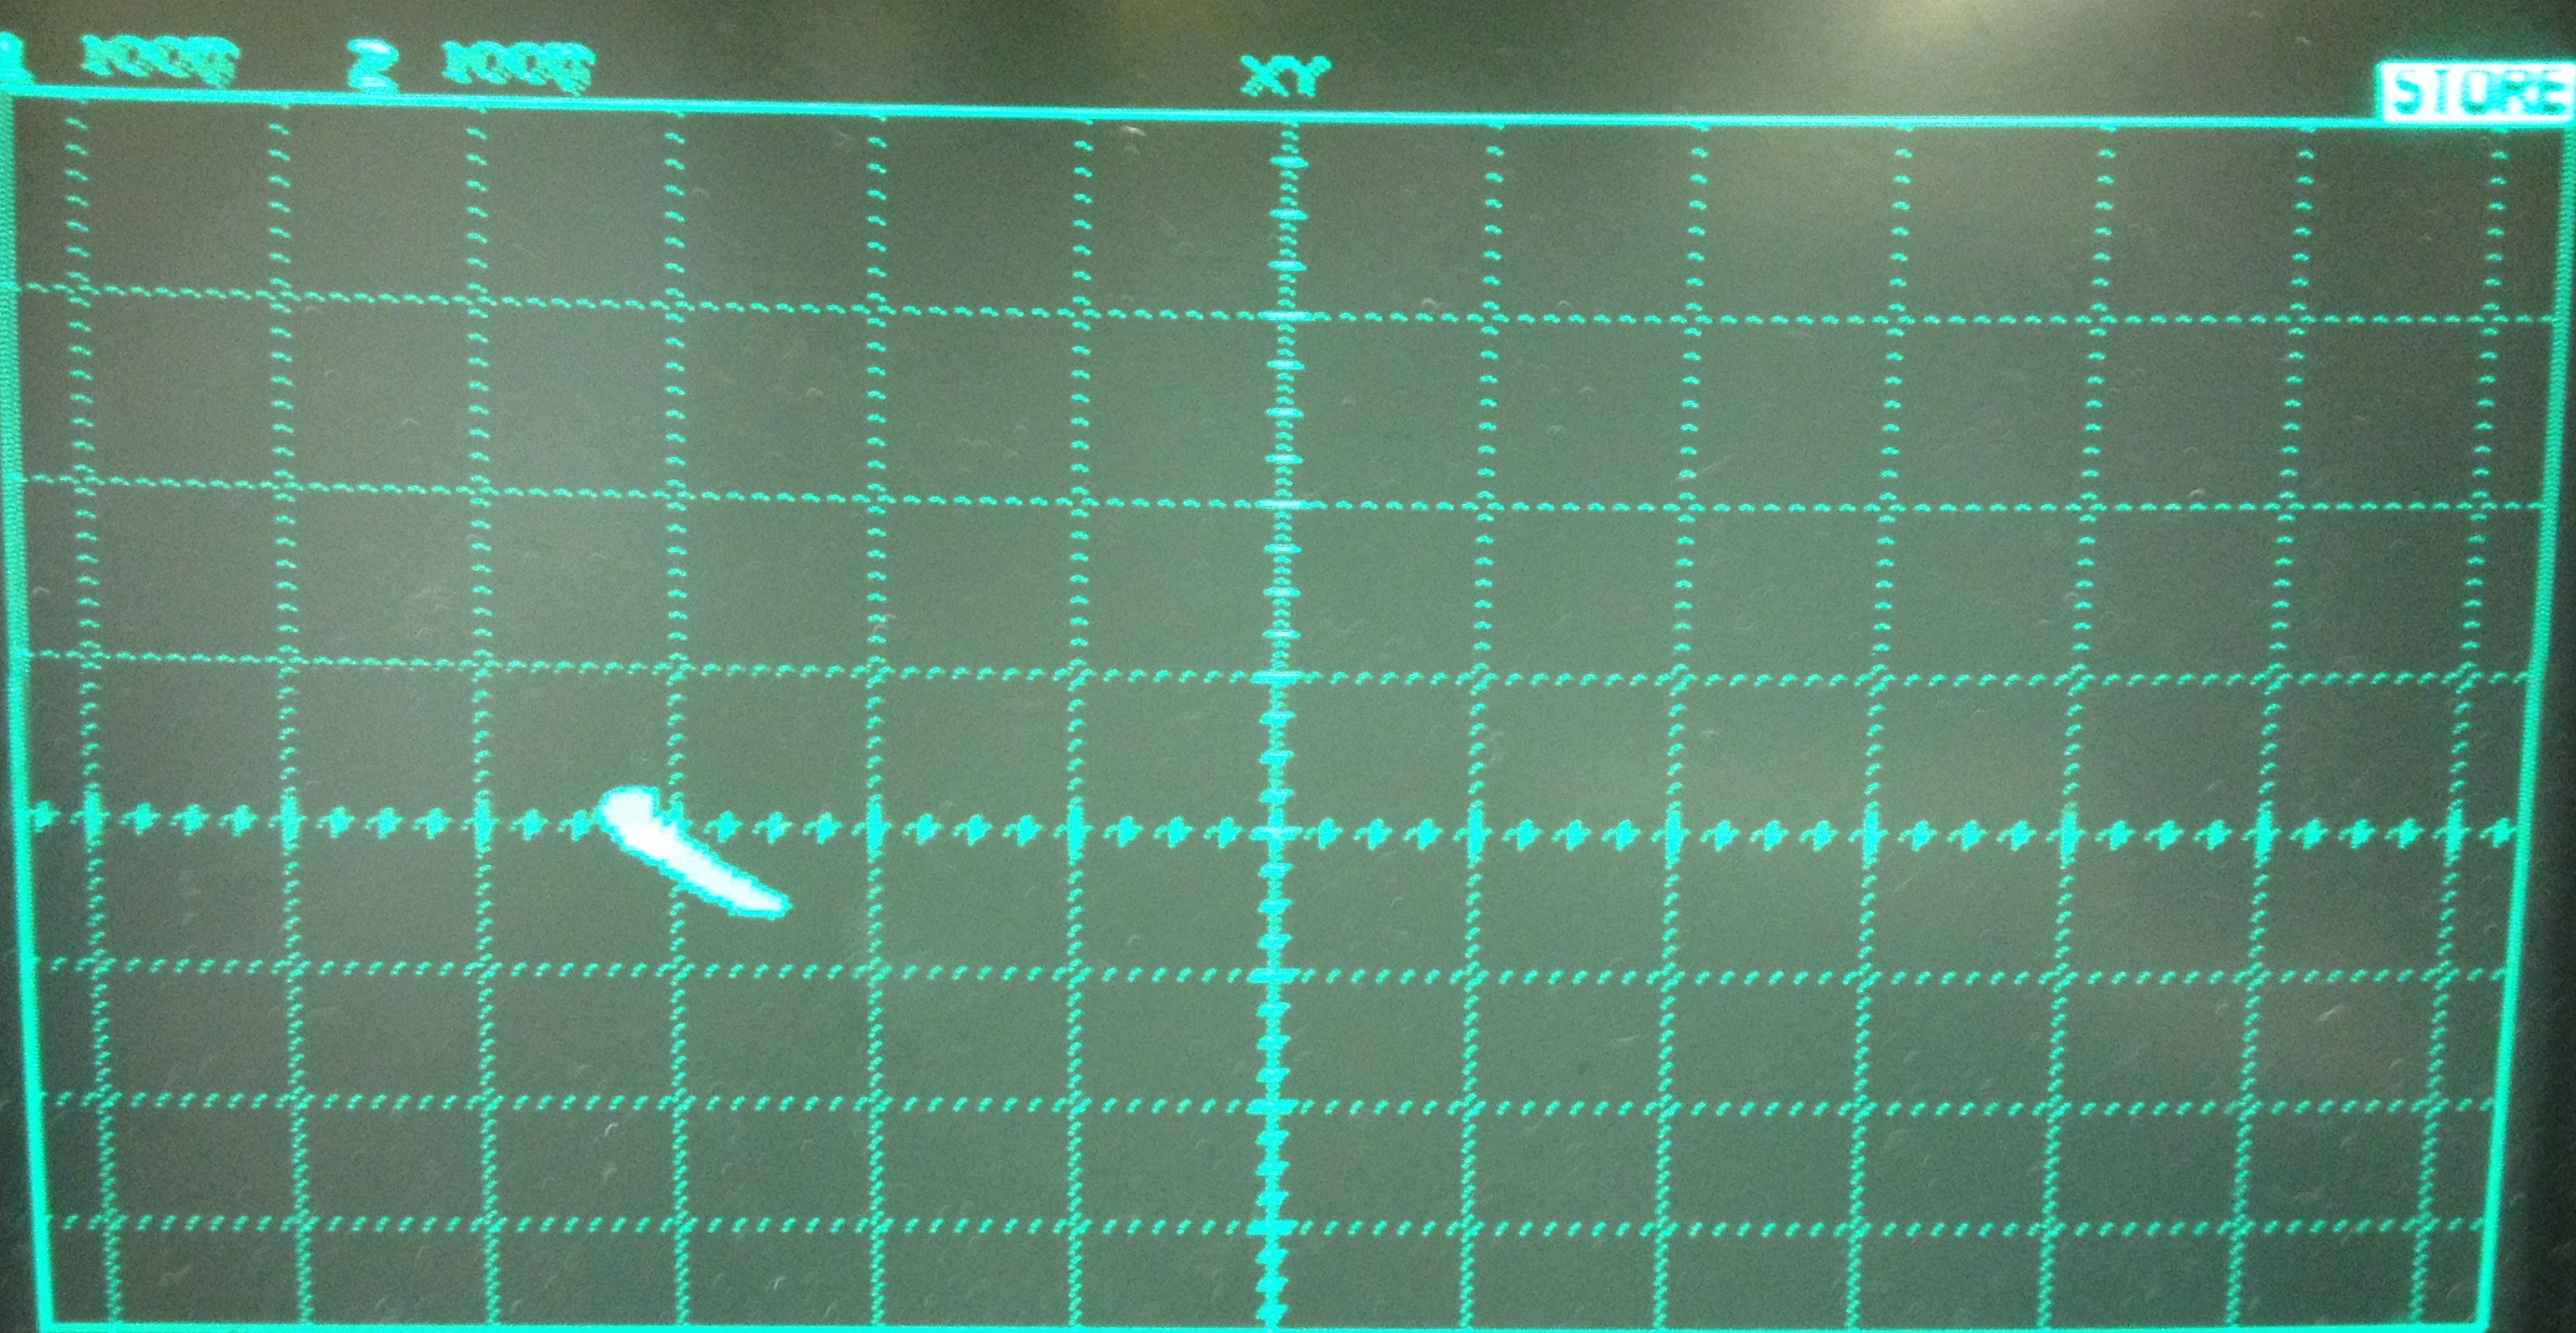
\includegraphics[width=0.5\linewidth,angle=0]{./figures/1T_1_18Hz.png}
%     }
%     % \hfill
%     \subfloat[$\omega=2\pi0.48$ [Hz] mouvement deux fois périodique.\label{fig:dipol2T}]{%
%       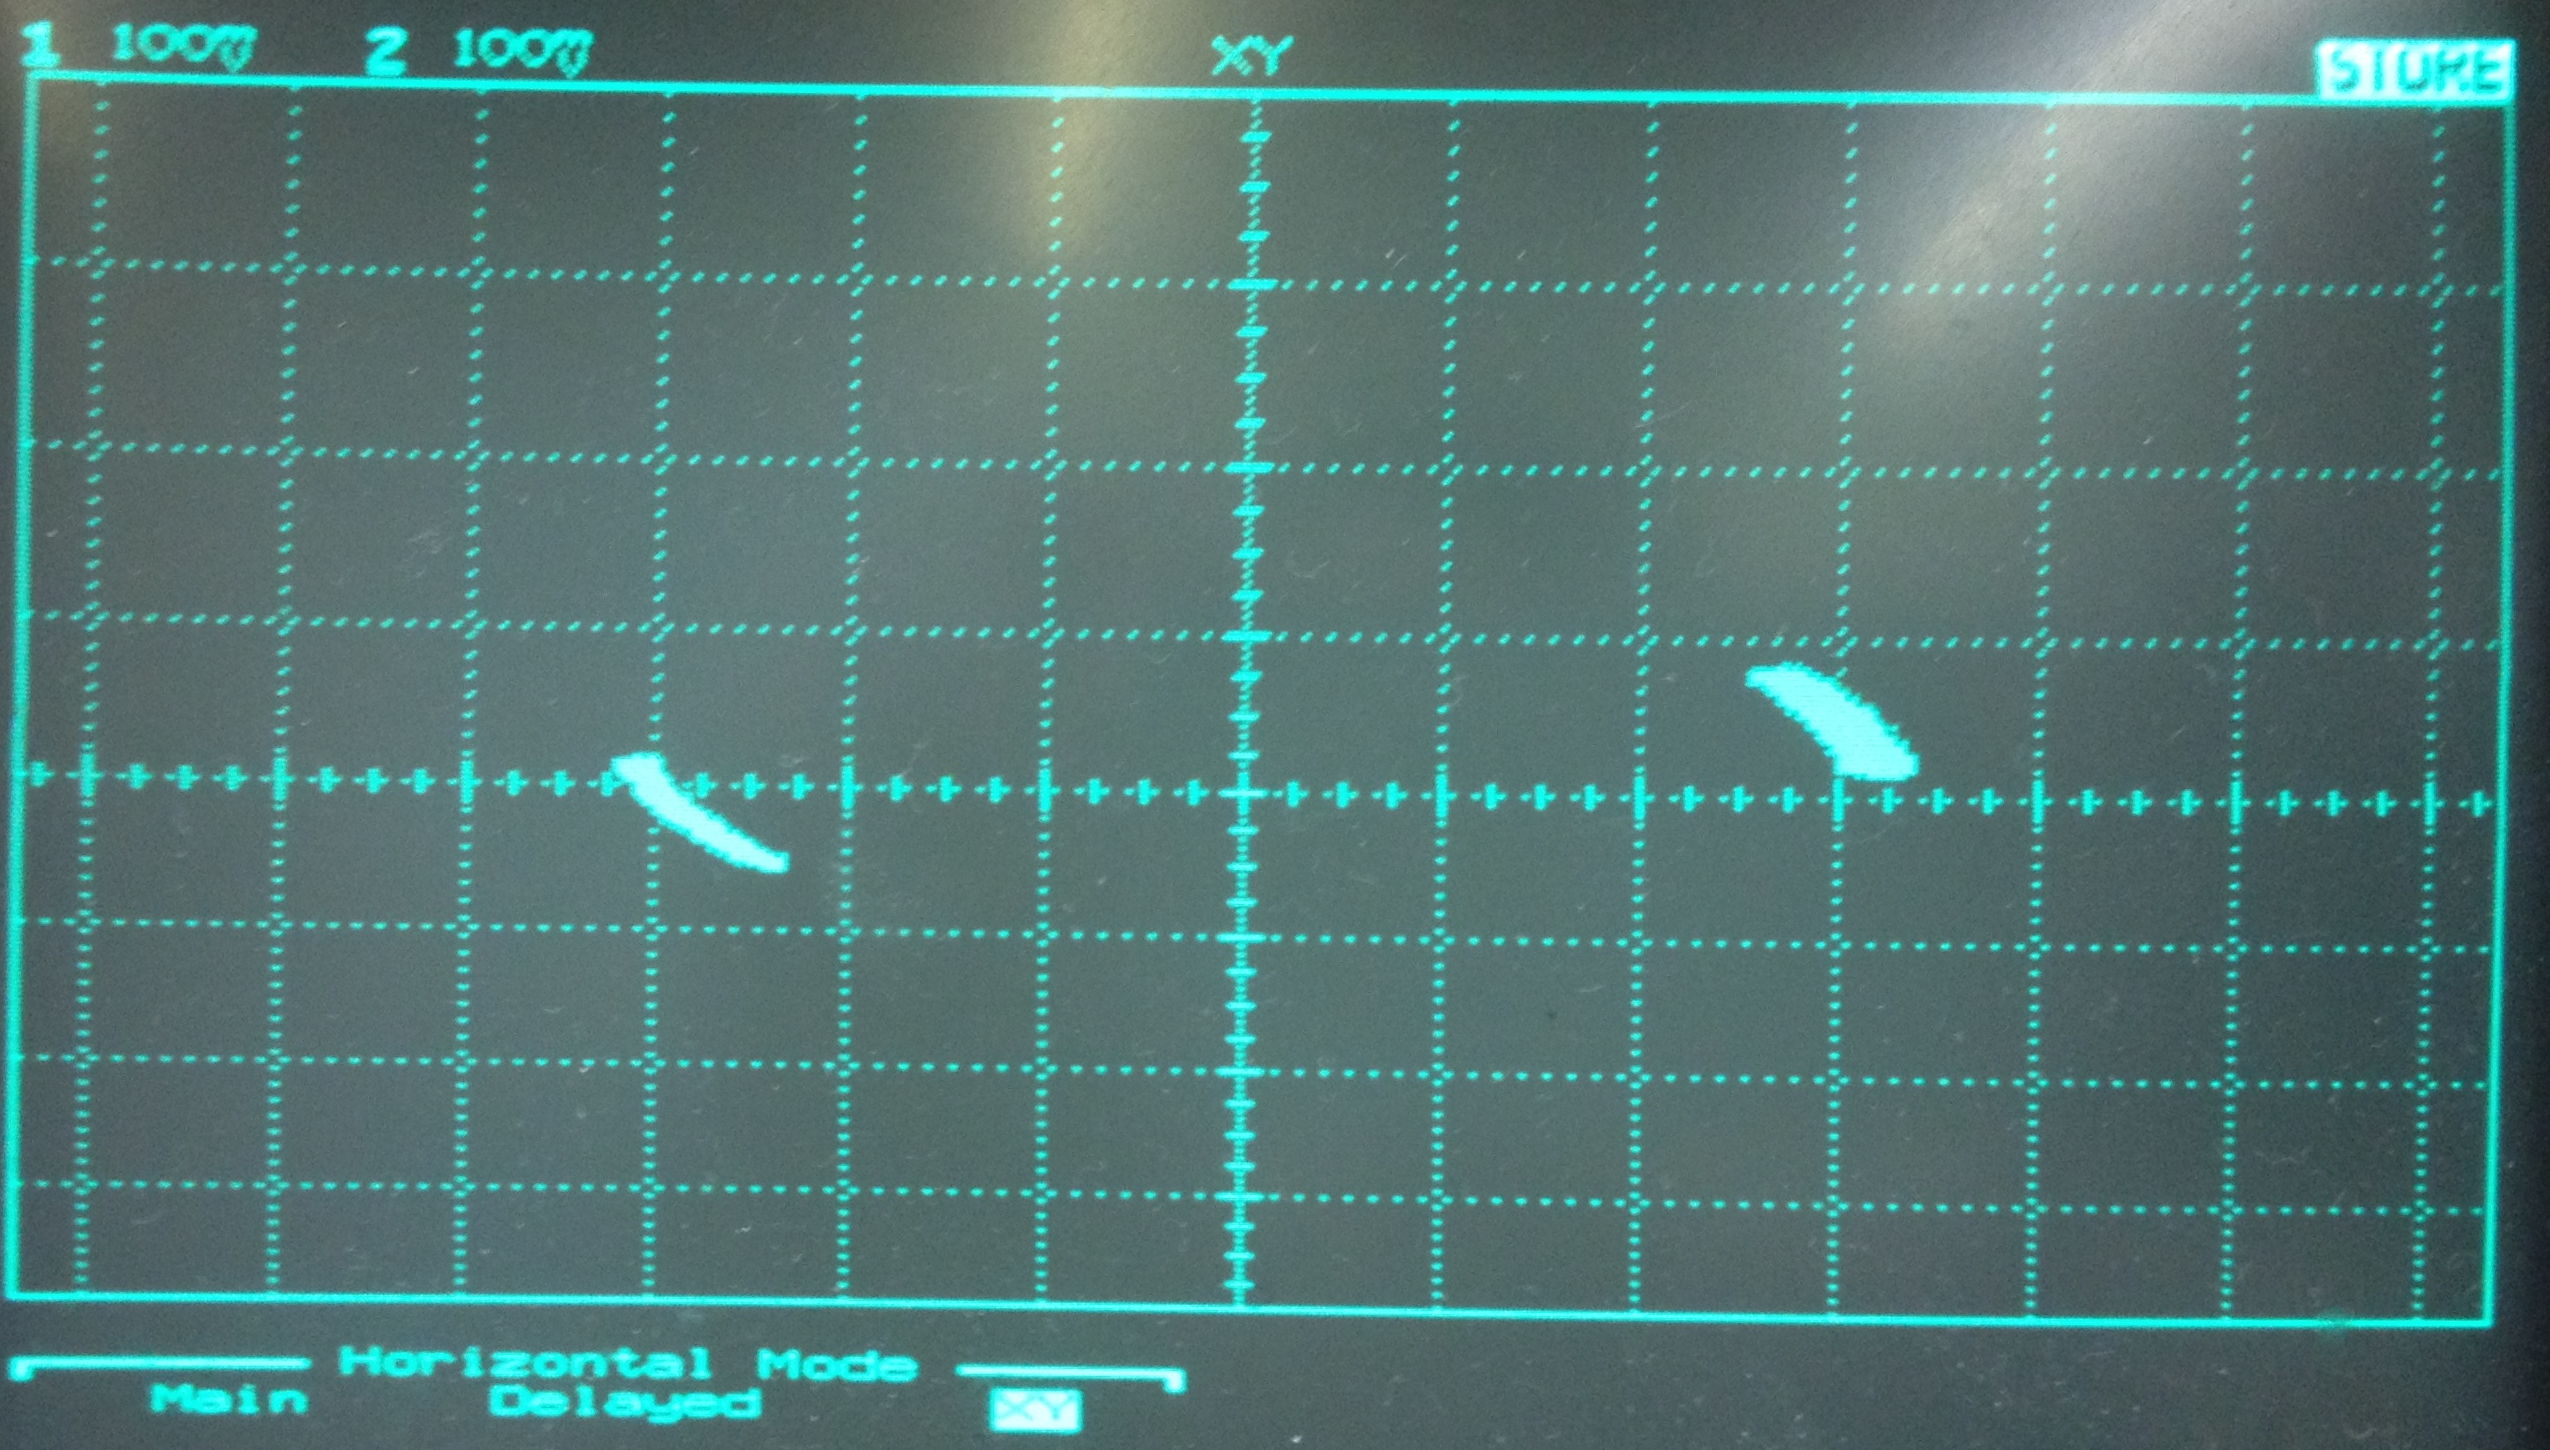
\includegraphics[width=0.5\linewidth,angle=0]{./figures/2T_0_48Hz.png}
%       }
%     \hfill
%     \subfloat[$\omega=2\pi1.22$ [Hz] mouvement chaotique.\label{fig:chaos}]{%
%       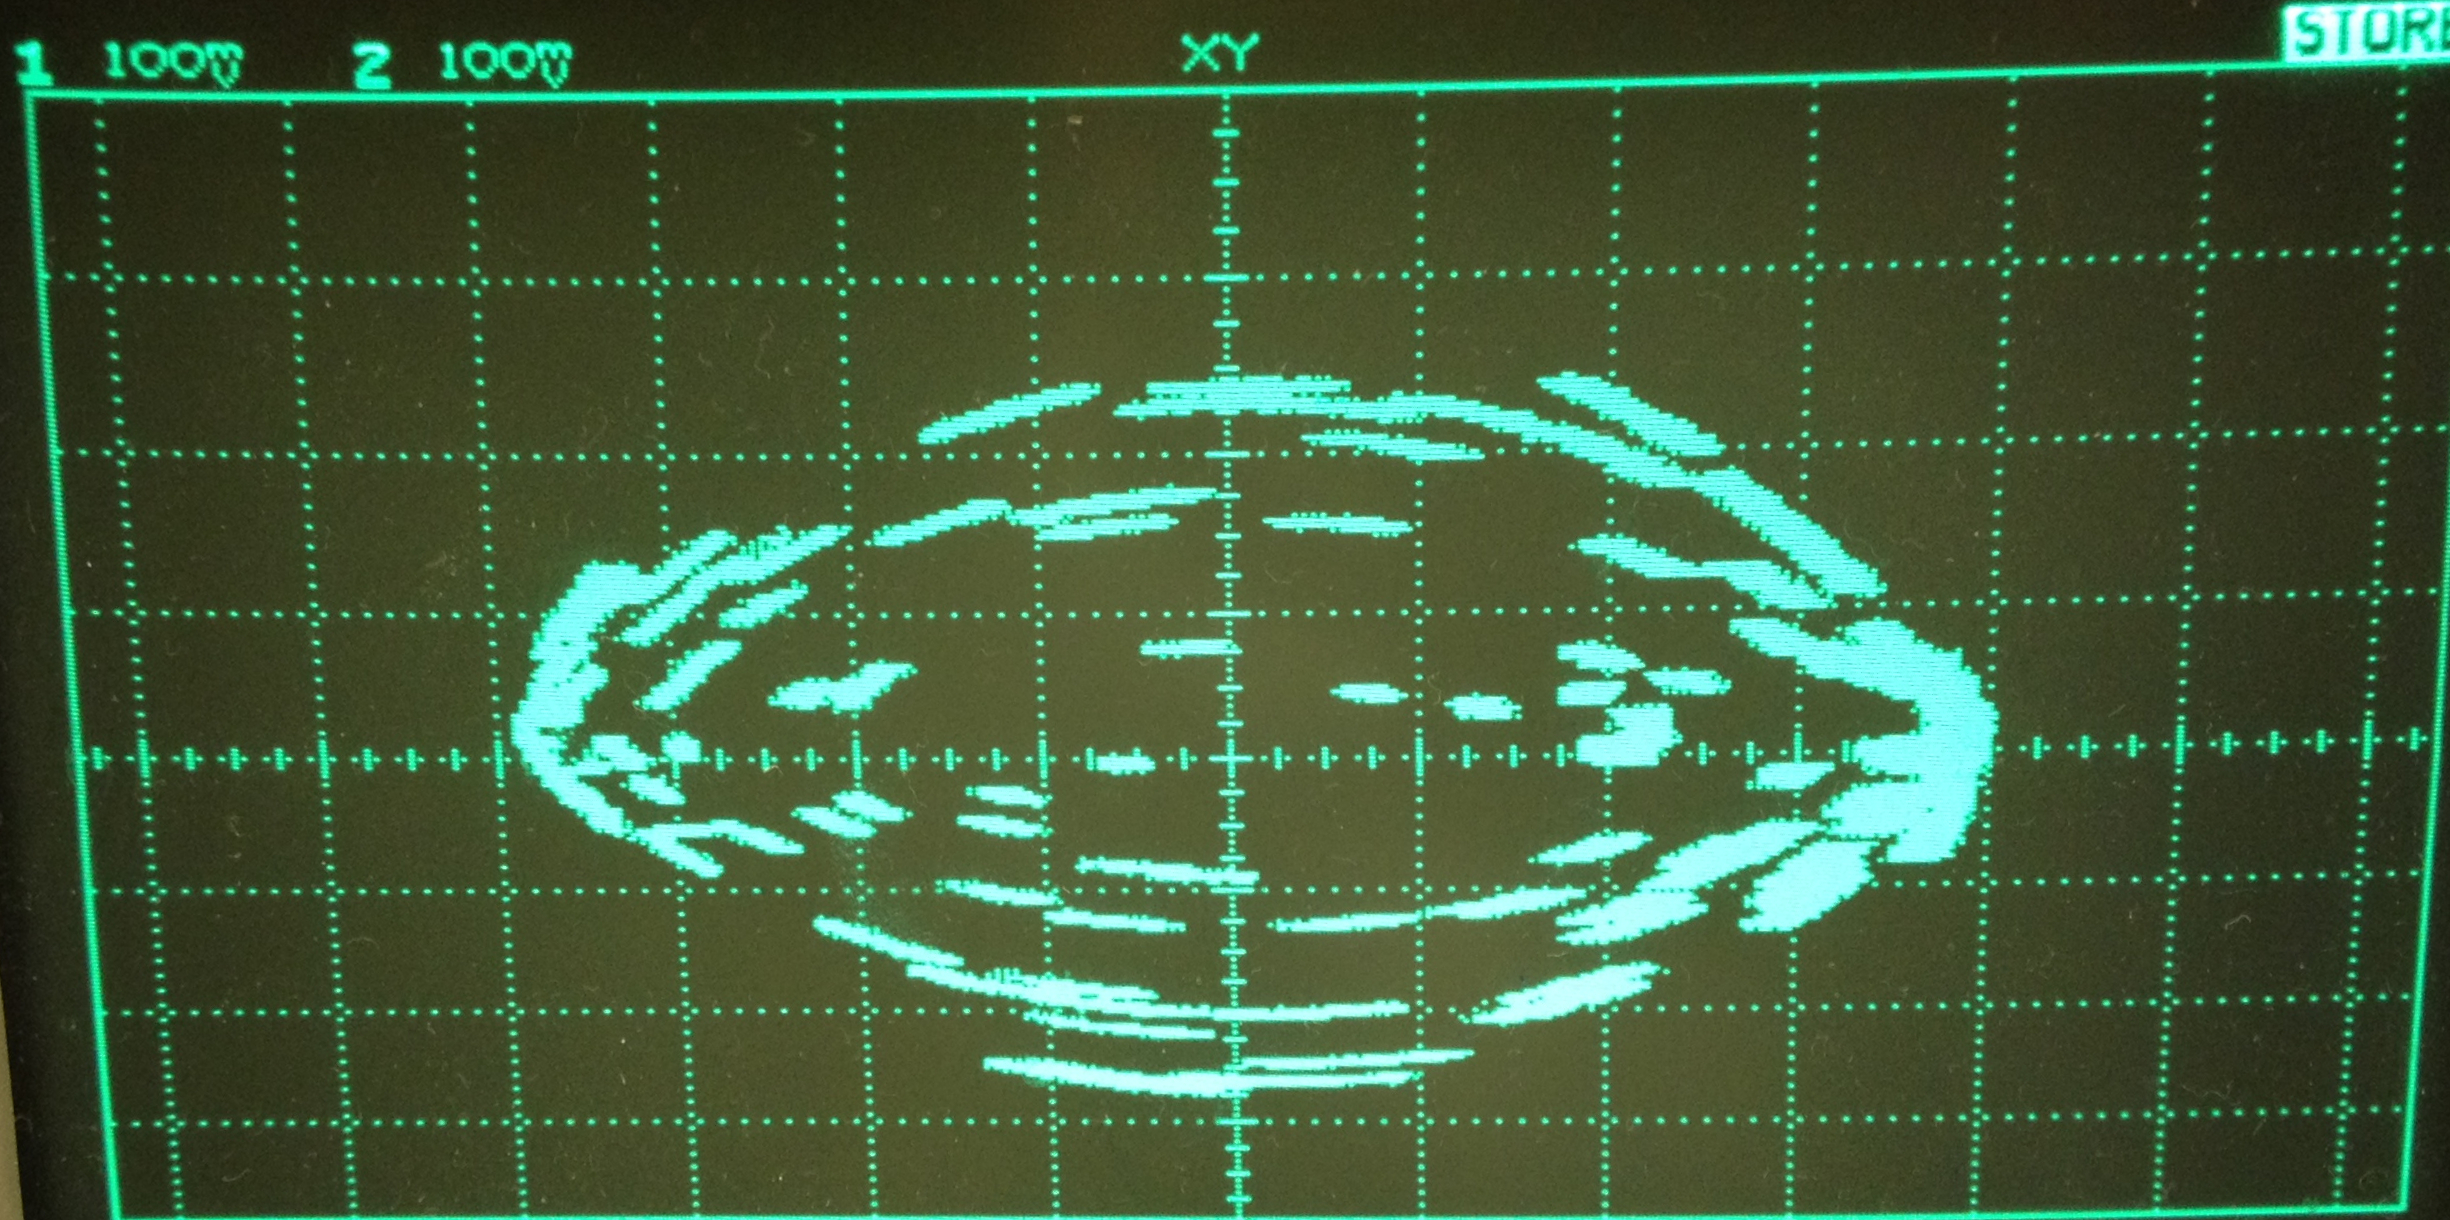
\includegraphics[width=0.5\linewidth,angle=0]{./figures/chao_1_22Hz_v2.png}
%     }
%     \caption{Sections de Poincaré}
%     \label{fig:poincare_section}
% \end{figure}

























\begin{figure}[!ht]
    \subfloat[f=0.486 \rm{[Hz]}\label{fig:a}]{%
      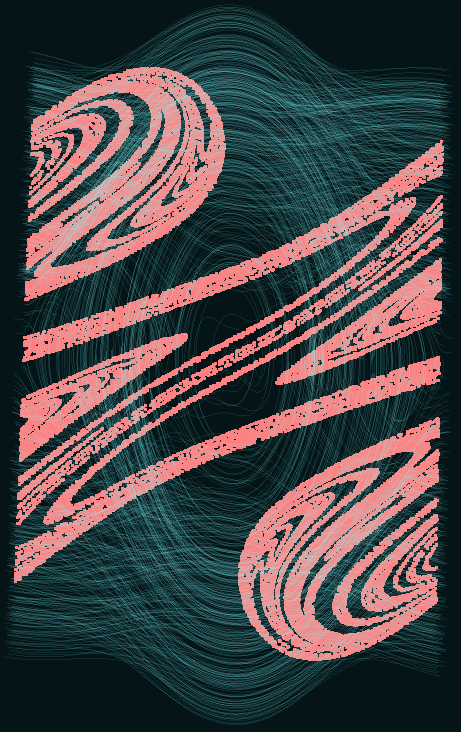
\includegraphics[width=0.5\textwidth]{./figures/poincare_beauty.png}
    }
    \hfill
    \subfloat[f=1.15 \rm{[Hz]}\label{fig:b}]{%
      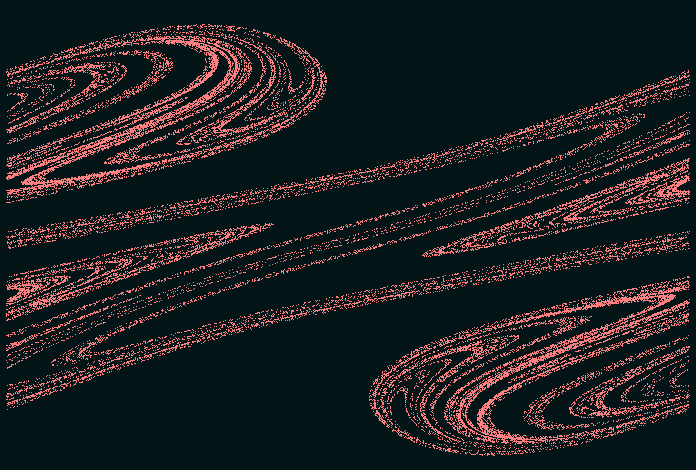
\includegraphics[width=0.5\textwidth]{./figures/poincare_beauty_2.png}
    }
    \hfill
    \subfloat[f=1.35 \rm{[Hz]}\label{fig:c}]{%
      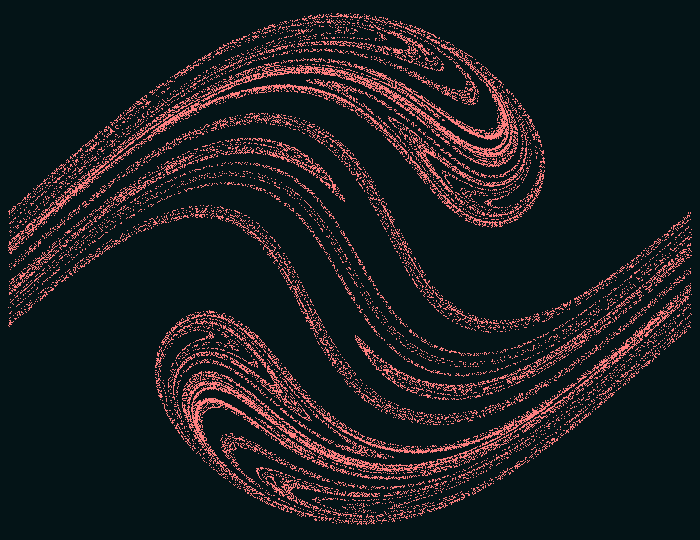
\includegraphics[width=0.5\textwidth]{./figures/poincare_beauty_3.png}
    }
    % \hfill
    % \subfloat[f=1.74 \rm{[Hz]}\label{fig:d}]{%
    %   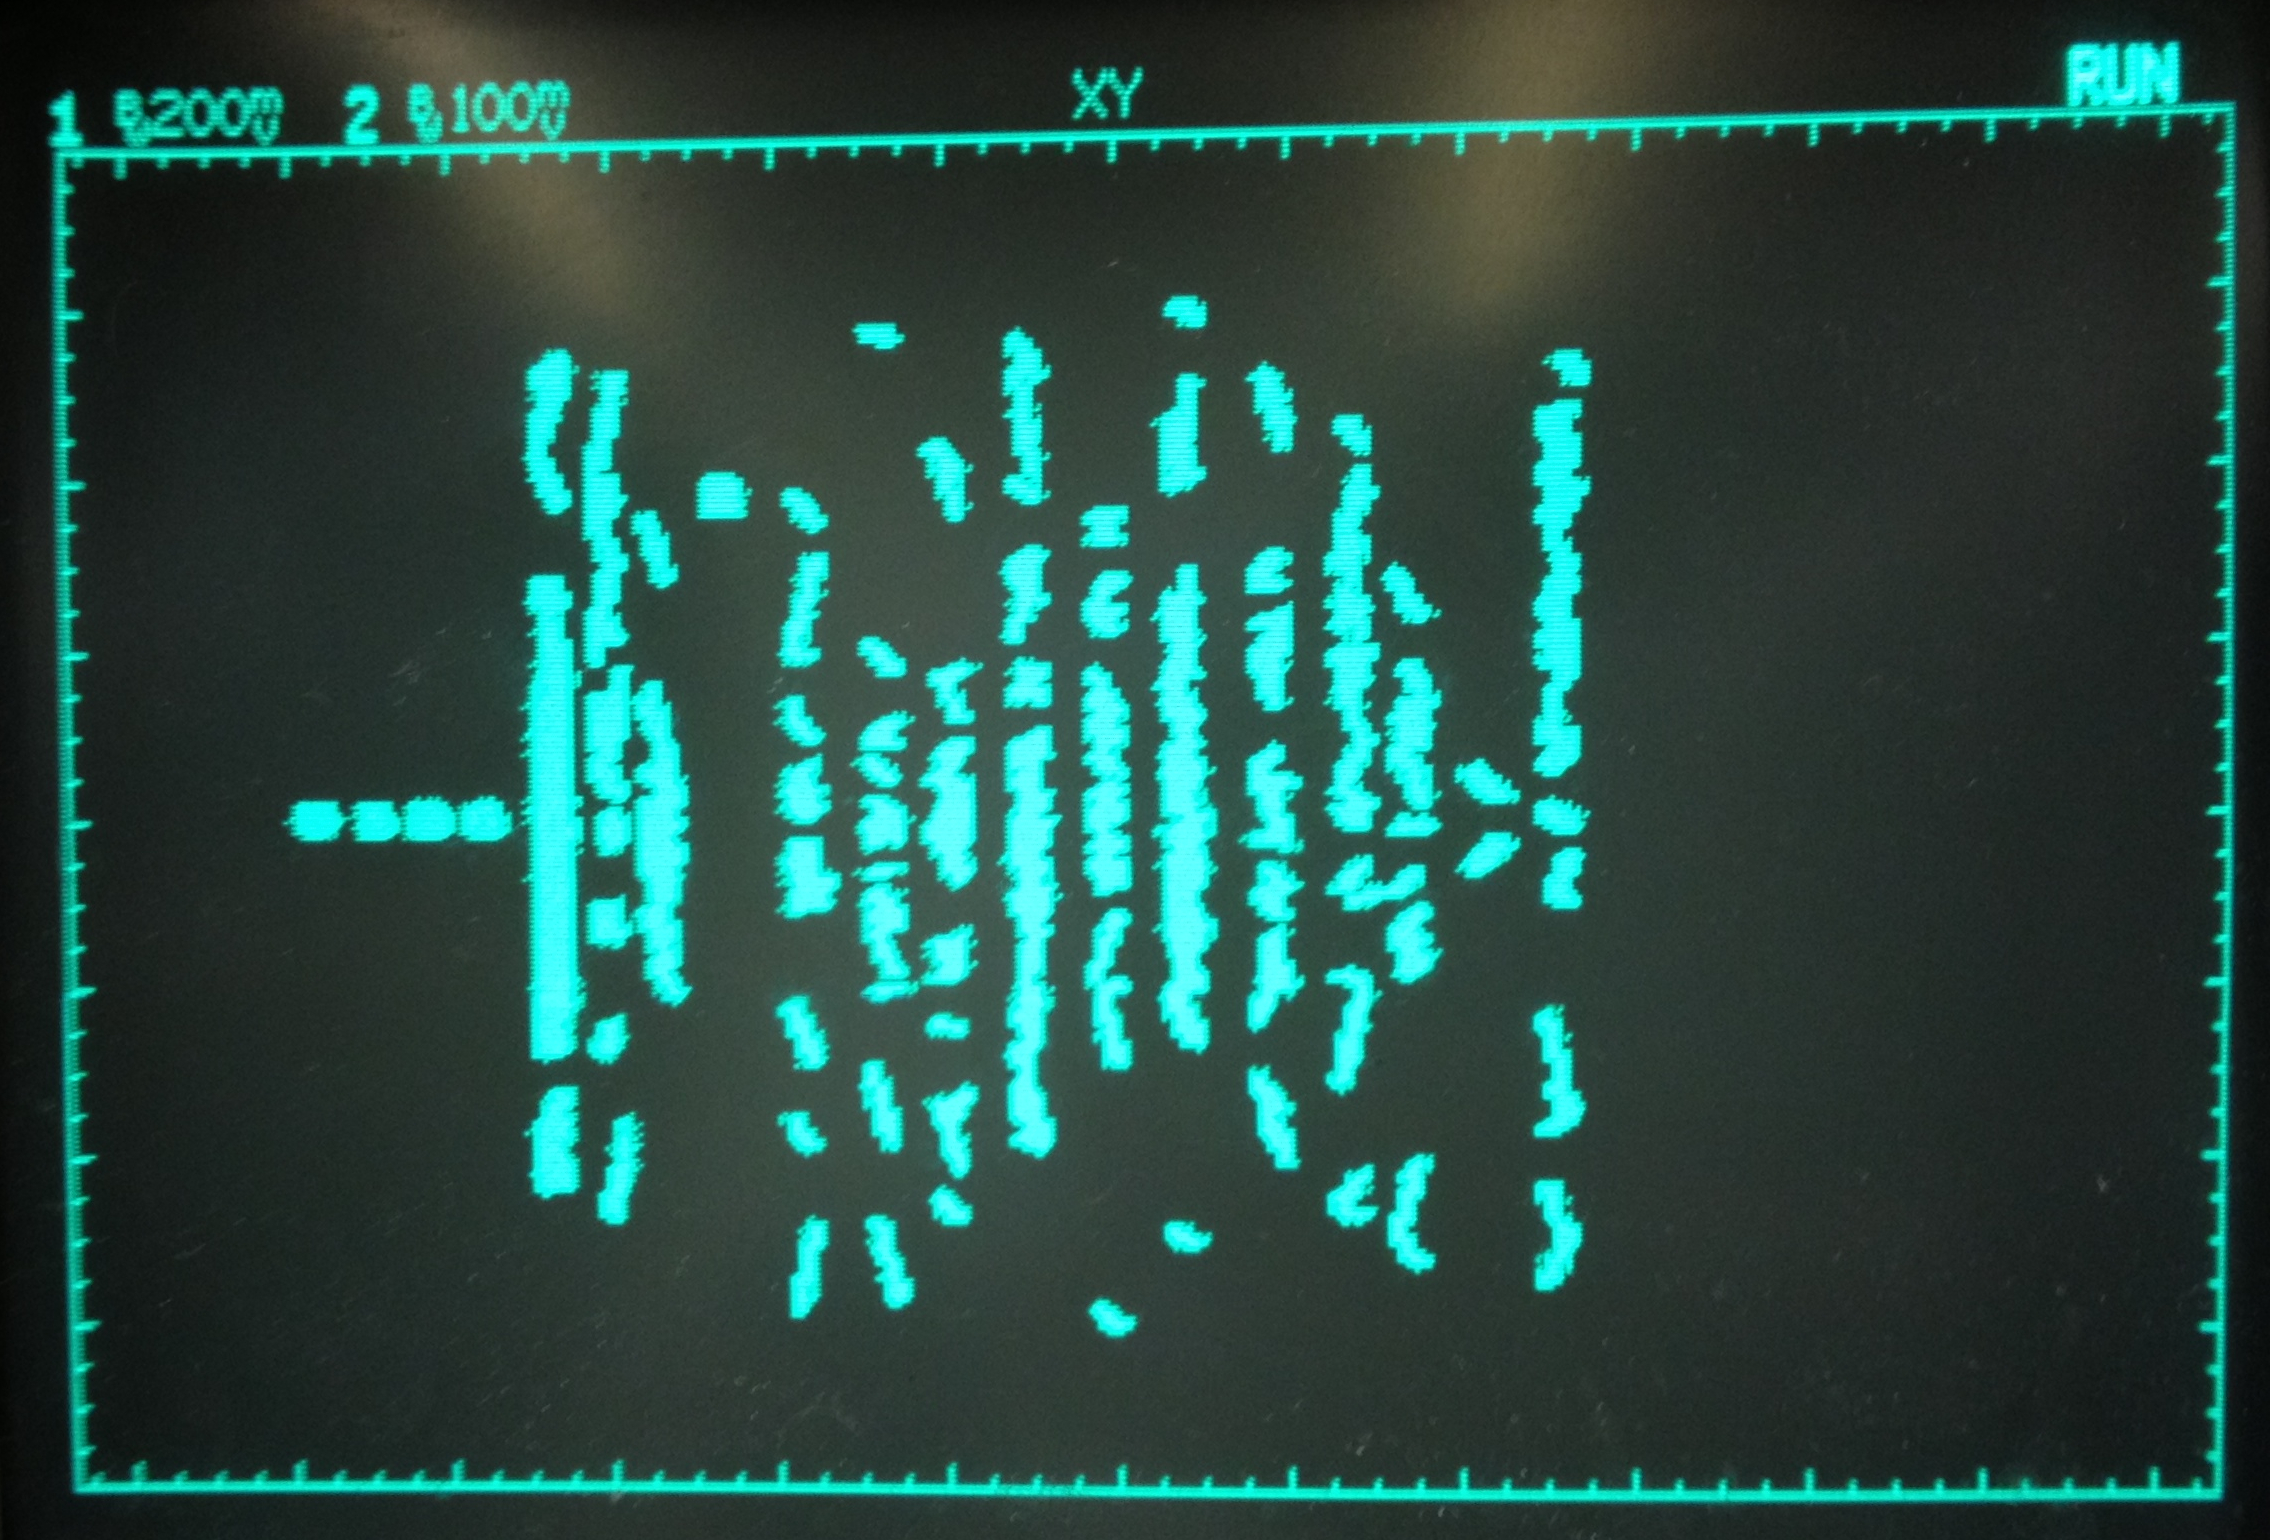
\includegraphics[width=0.5\textwidth]{./figures/bif_1_74Hz.png}
    % }
    \caption{Il a été simulé à l'ordinateur la même expérience afin d'obtenir des setions de Poincaré plus fine, en voici quelques unes, disons juste pour nous rincer l'oeil ! La premiere montre en transparance la trajectoire du pendule. Nous n'avons malheureusement pas eu le temps de faire un diagramme de bifurcation avec notre code.}
    \label{fig:poincare_beauty}
\end{figure}

Pour la réalisation des diagrammes de bifurcations fonction de $F$, il a d'abord été tenté une variation sur $\omega$, ce qui aboutit à une transformation compliquée pour retrouver l'allure du diagramme de bifurcation. Il a finalement été réalisé des diagrammes en itérant sur l'amplitude du champ magnétique (cf section \ref{description}).

Pour obtenir de bons diagrammes de bifurcations, il faut faire attention à ce qu'on prenne des mesures sur la position du pendule dans l'espace de phase lorsque celui ci s'est rapproché au maximum d'un attracteur car si le système est en transition, il ne sera pas possible d'observer d'orbites et la tranche du diagramme de bifurcation obtenue ne sera pas distinguable d'un cas chaotique.

Dans la série de graphes de \ref{fig:bifurcation}, il a été produit des diagrammes de bifurcations pour 4 valeurs de $\omega$ constantes. Il a été assez difficile de trouver des mesures pour lesquelles le pendule se trouve dans une dynamique non chaotique. On peut voir dans le diagramme d deux zones correspondant à des orbites simples, et une autre zone ou le pendule oscille dans deux orbites. 

\begin{figure}[!ht]
    \subfloat[$\omega$=2 $\pi$ 0.486 \rm{[Hz]}\label{fig:a}]{%
      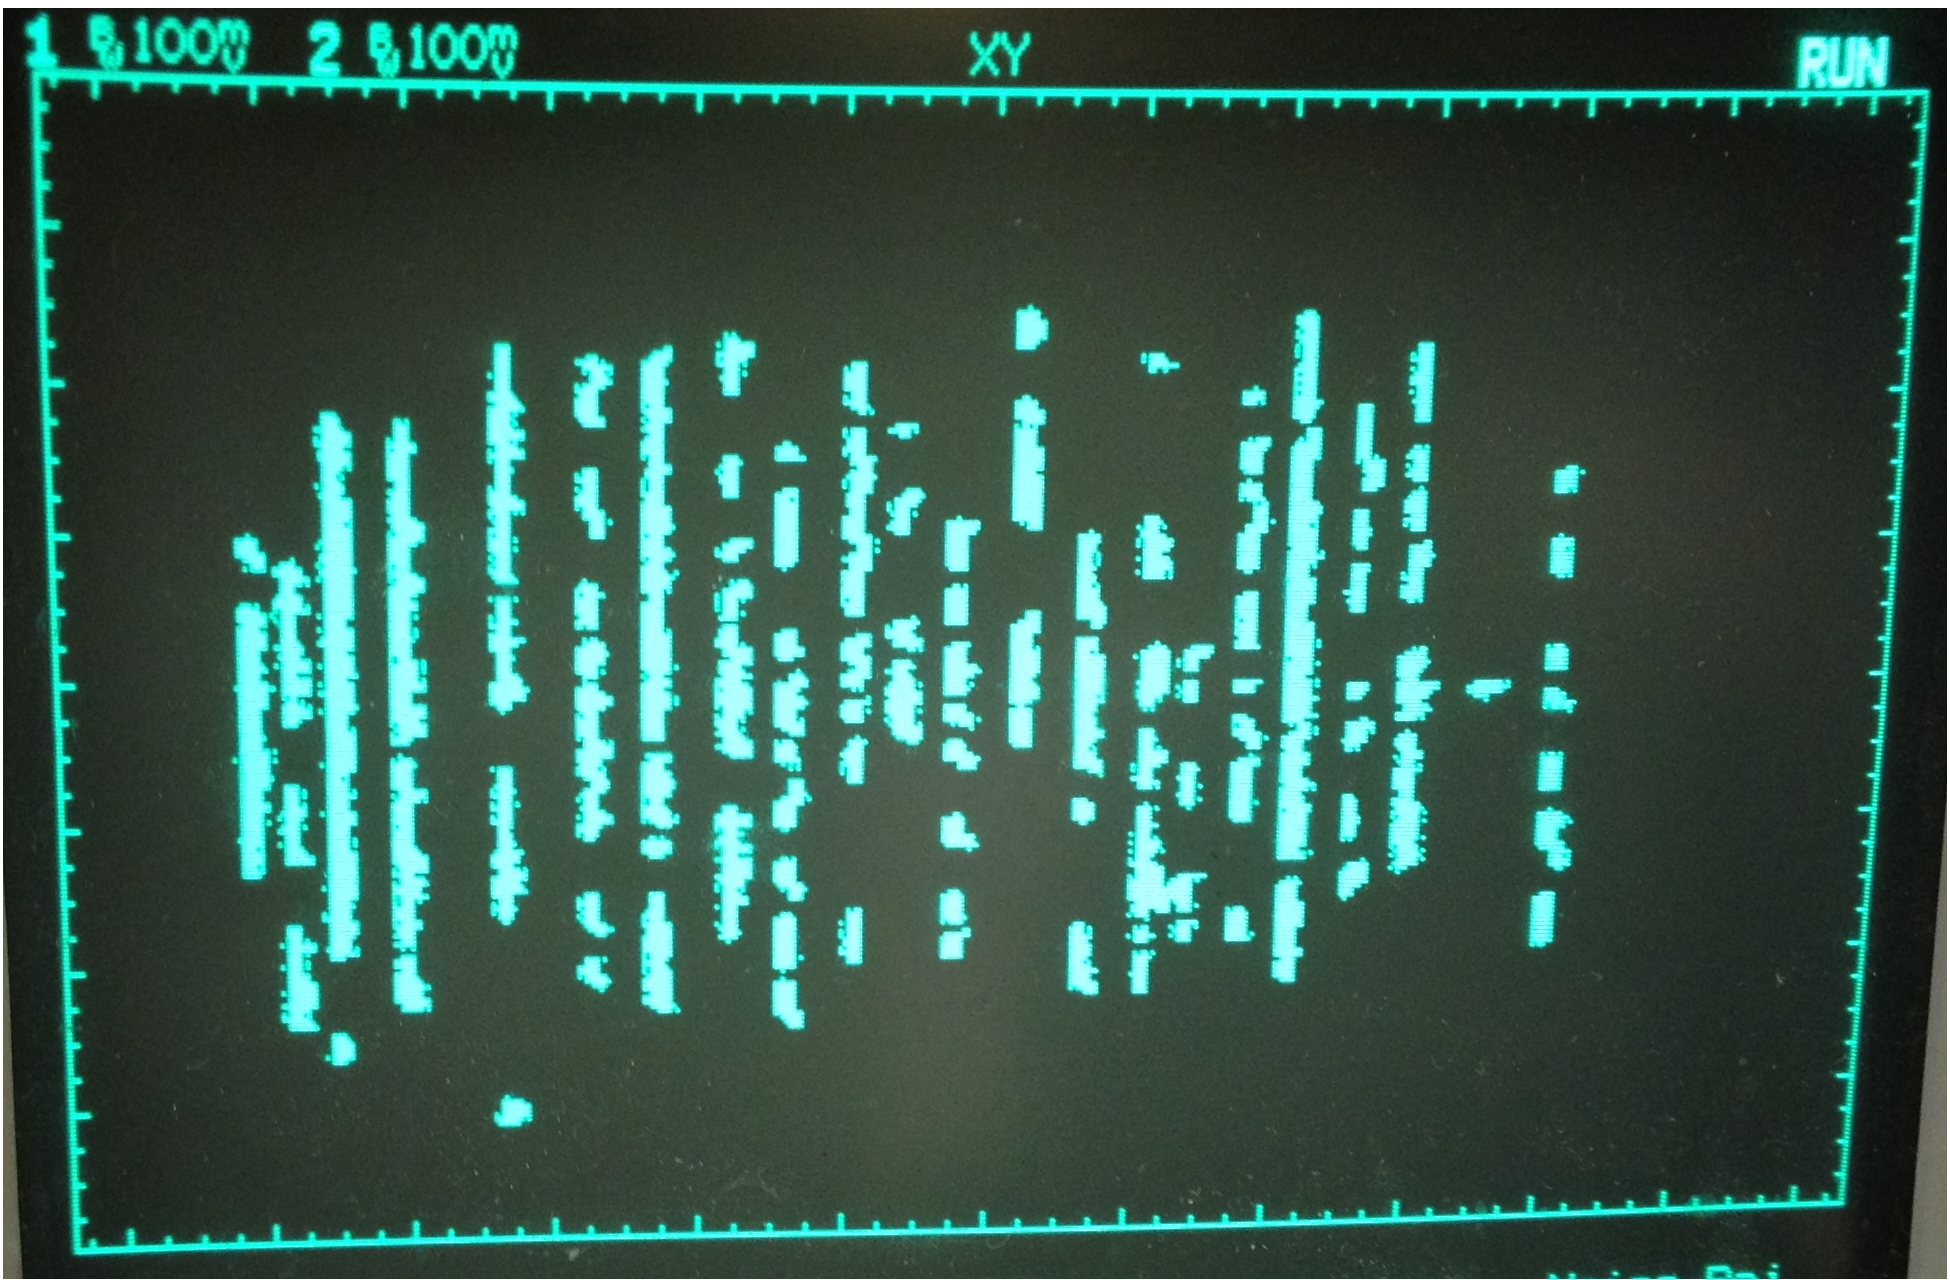
\includegraphics[width=0.5\textwidth]{./figures/bif_0_486Hz.png}
    }
    \hfill
    \subfloat[$\omega$=2 $\pi$ 1.15 \rm{[Hz]}\label{fig:b}]{%
      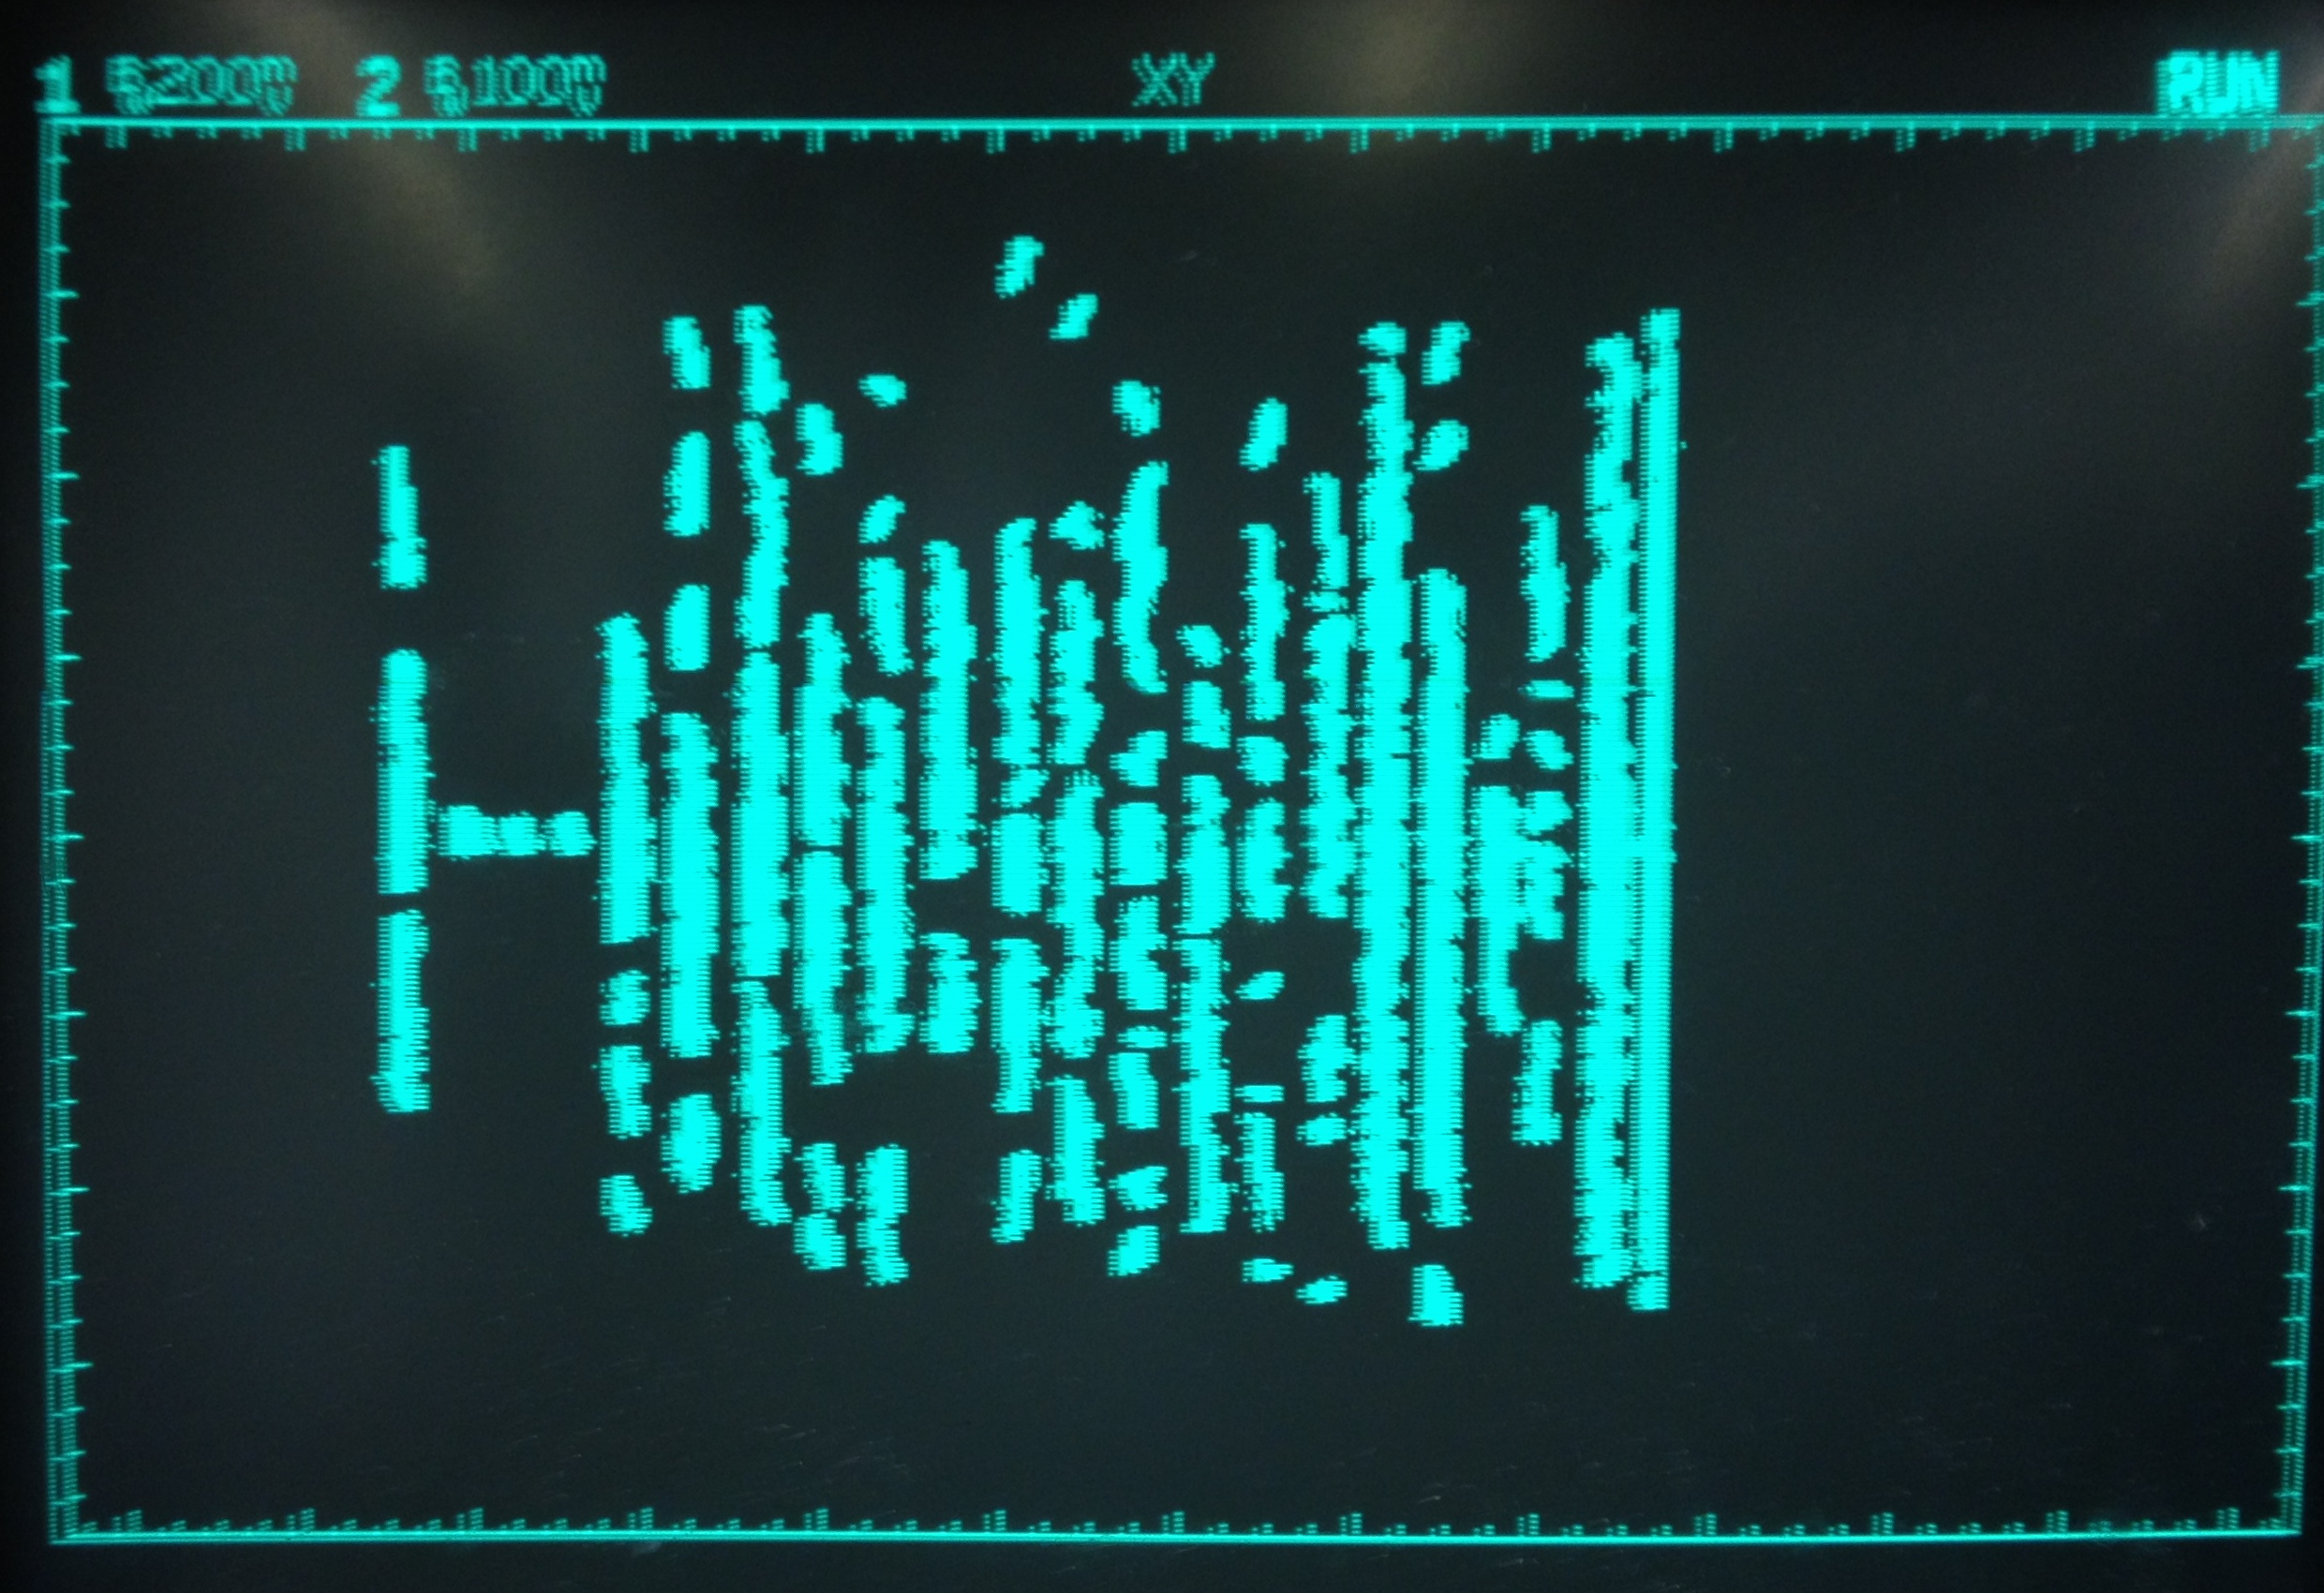
\includegraphics[width=0.5\textwidth]{./figures/bif_1_15Hz.png}
    }
    \hfill
    \subfloat[$\omega$=2 $\pi$ 1.35 \rm{[Hz]}\label{fig:c}]{%
      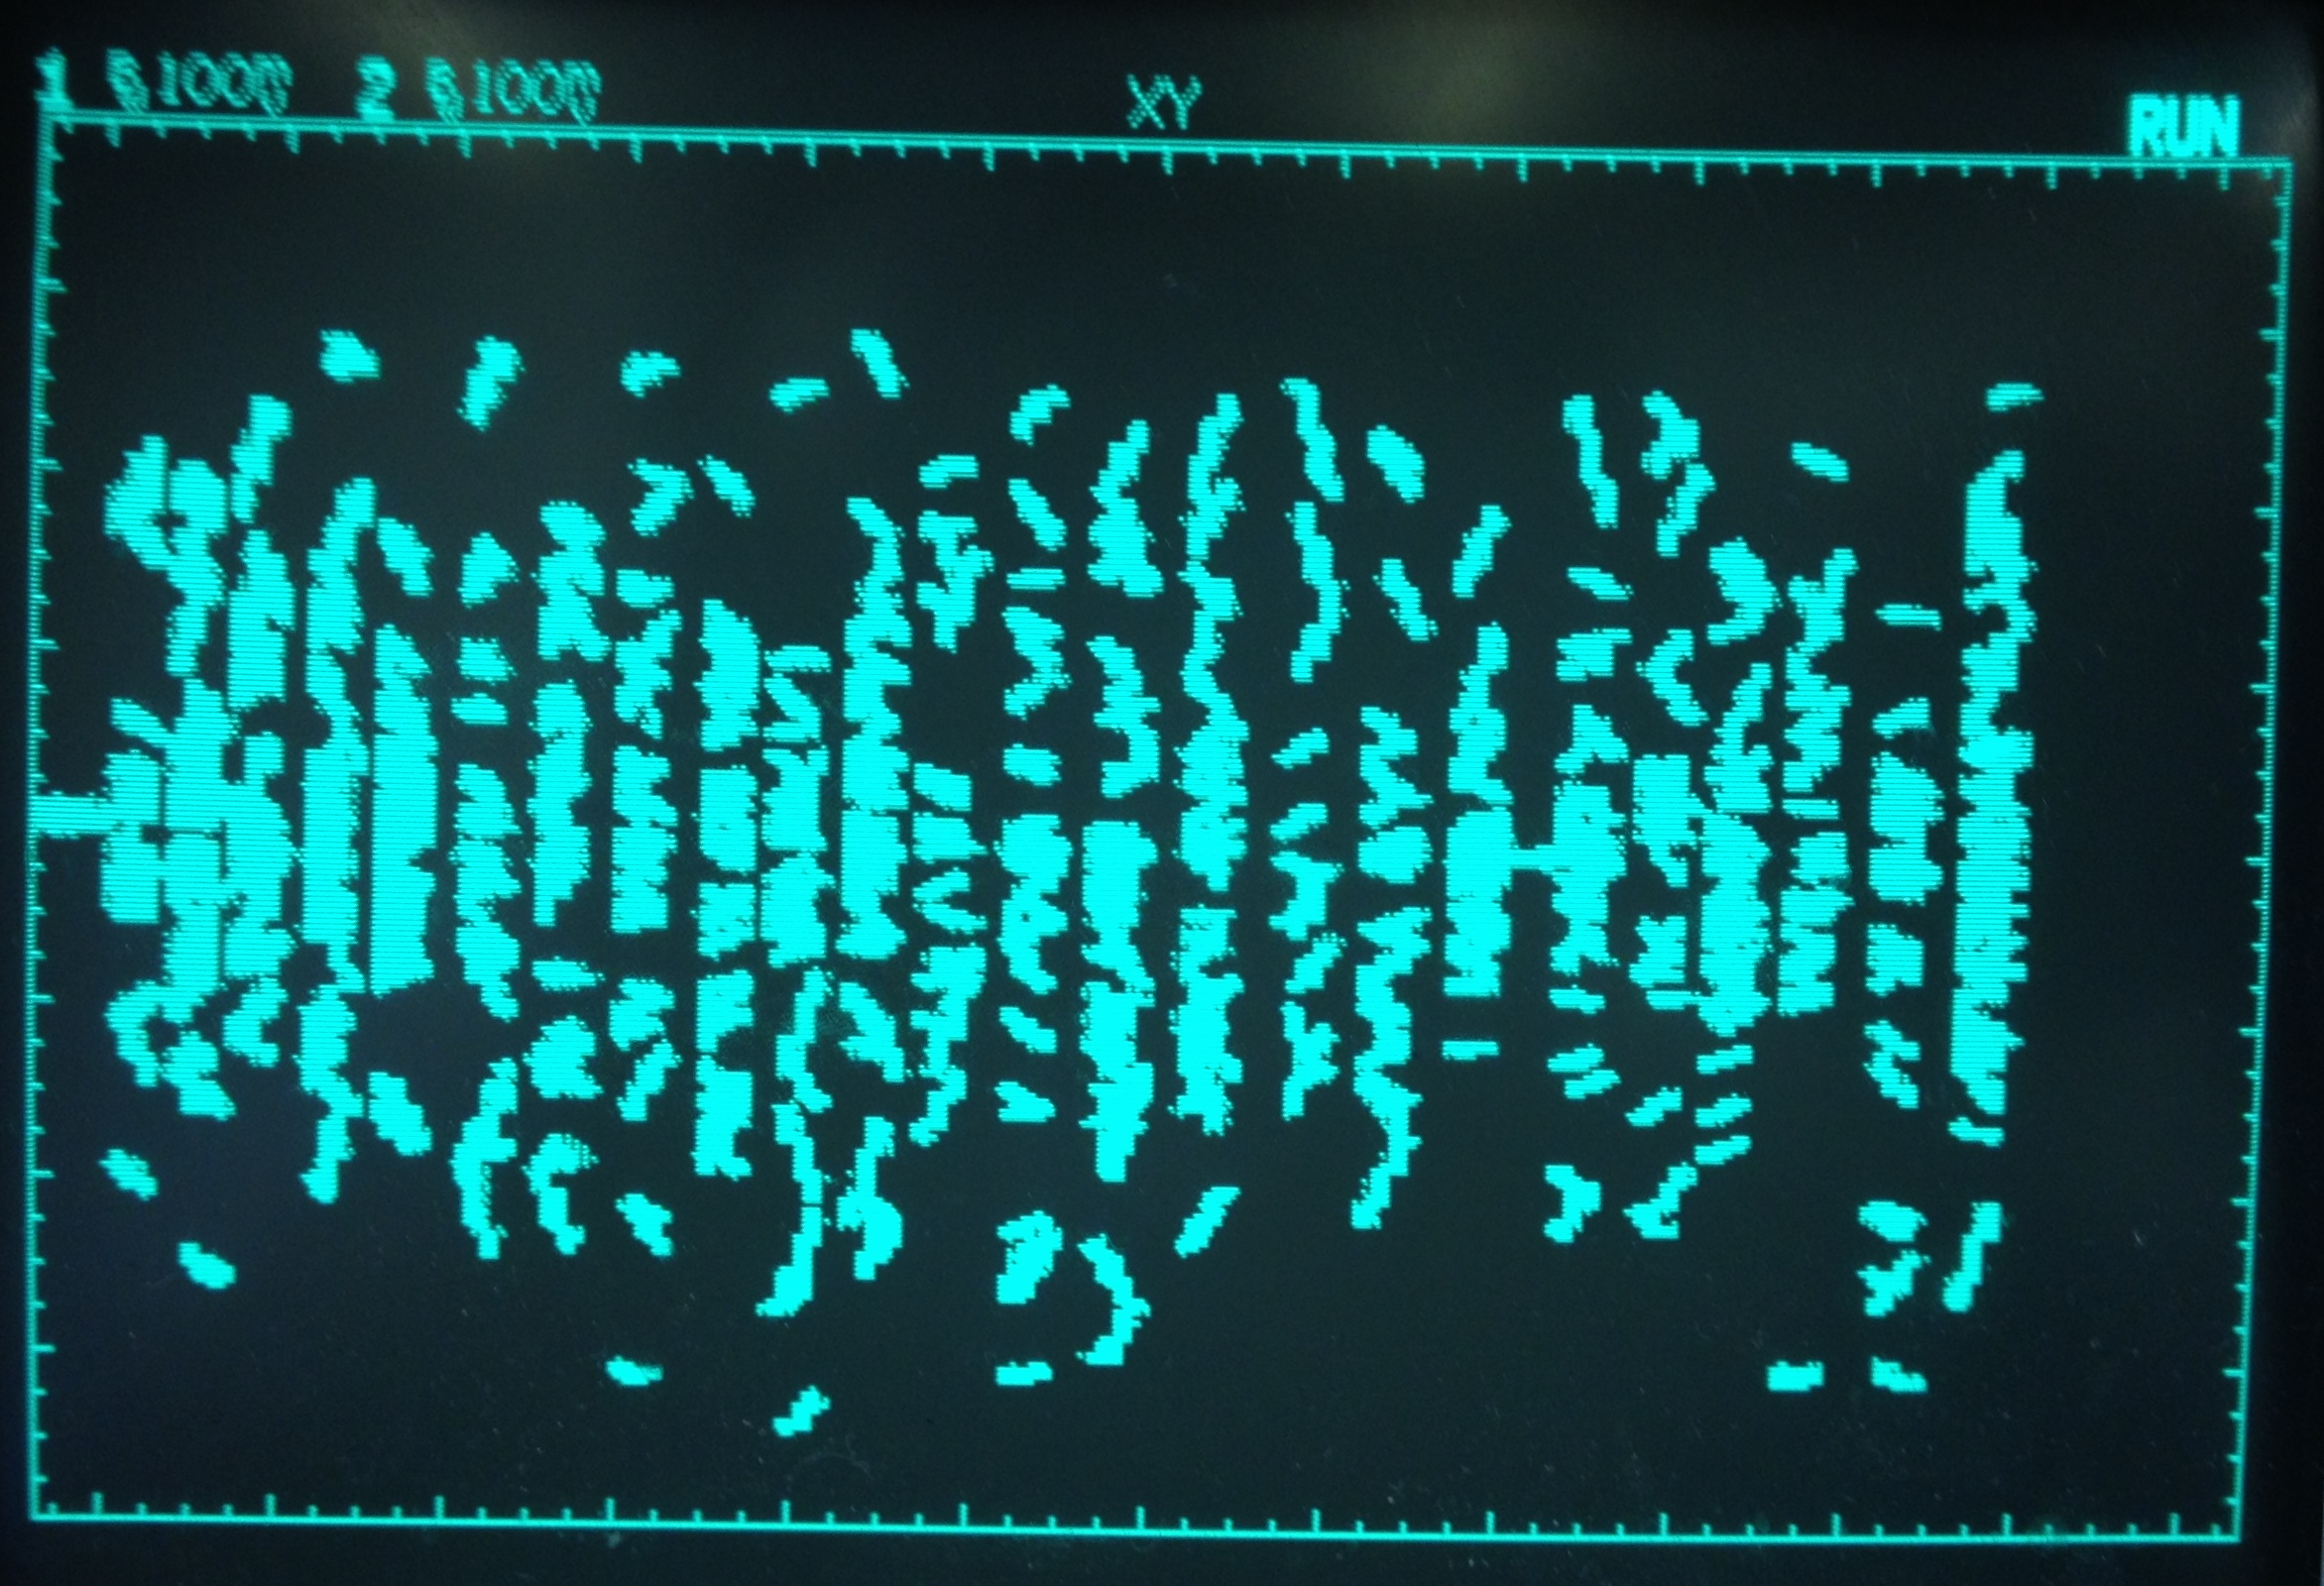
\includegraphics[width=0.5\textwidth]{./figures/bif_1_35Hz.png}
    }
    \hfill
    \subfloat[$\omega$=2 $\pi$ 1.74 \rm{[Hz]}\label{fig:d}]{%
      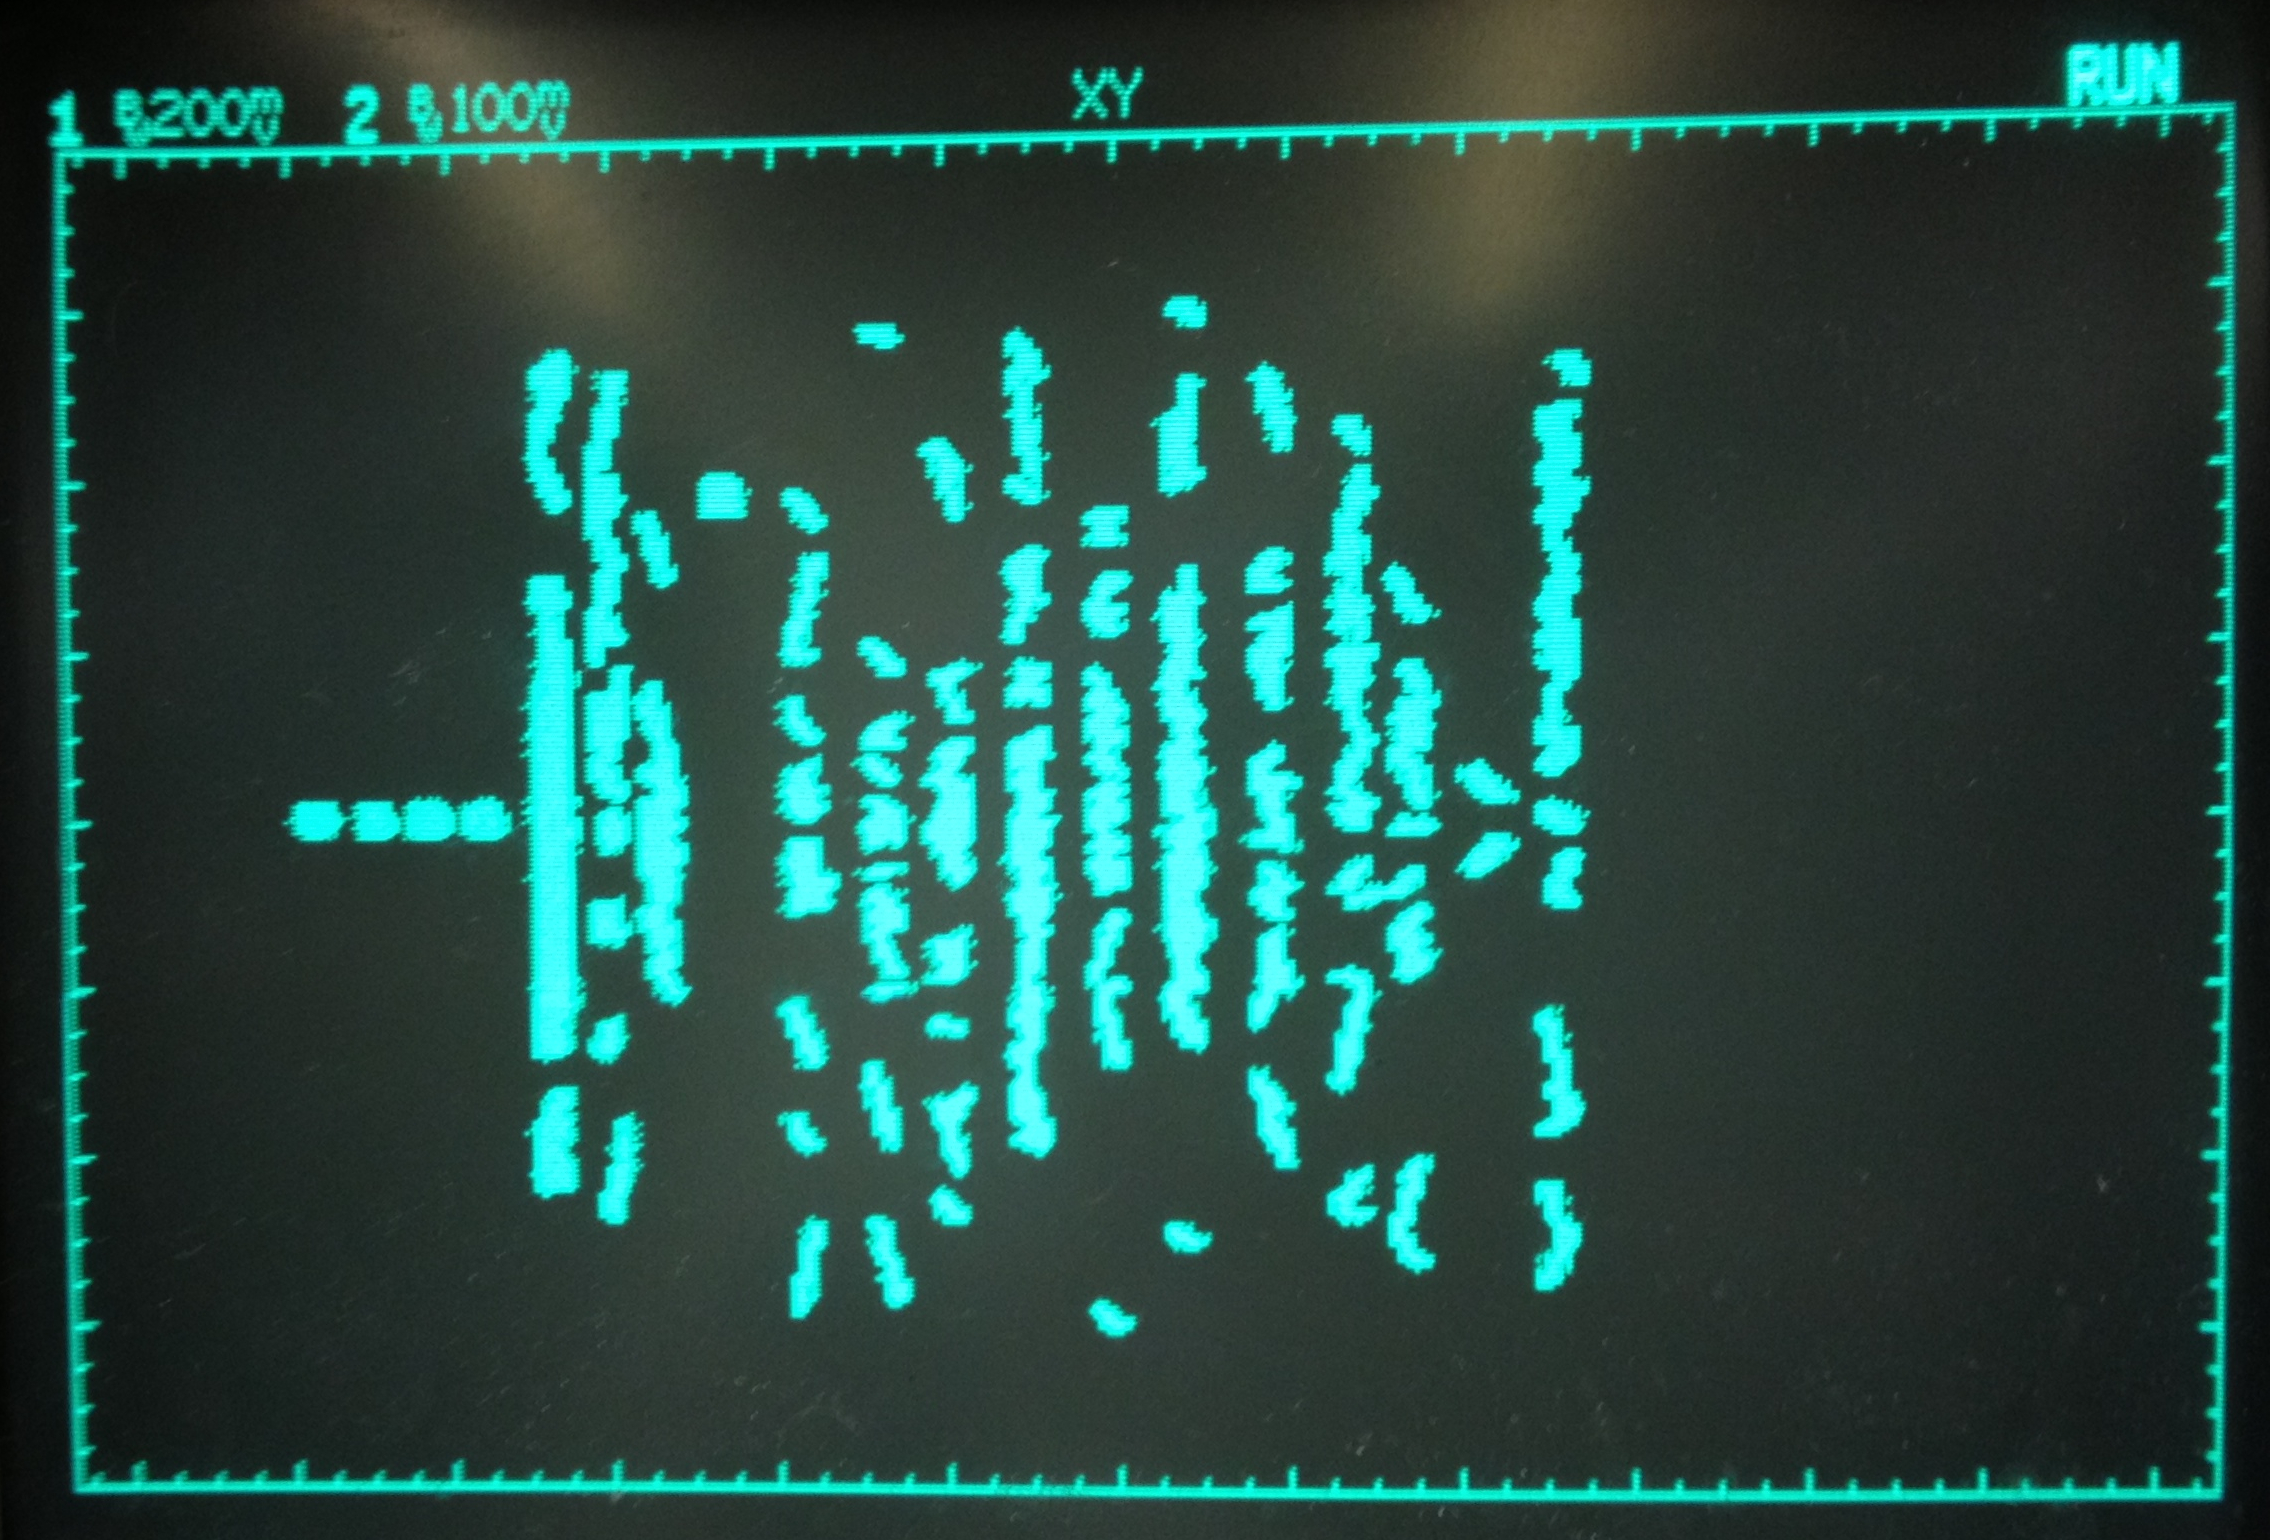
\includegraphics[width=0.5\textwidth]{./figures/bif_1_74Hz.png}
    }
    \caption{Bifurcation}
    \label{fig:bifurcation}
\end{figure}

% \newpage











\clearpage
\section{TODO FEST !!!! OMG OMG OMG OMG OMG OMG OMG OMG OM}


expliquer qu'il faut attendre un certain temps pour que le systeme approche de l'attracteur pour la construction du diagramme de bifurcations

type de mouvement

probleme du montage avec pendule inverse :
dessiner le potentiel au cours du temps
potentiel -> probleme de la symetrie

simulation

de jolis shemas

origine section poincare ?

conditions initiales
asteroides

% \newpage












\clearpage
\section{Analyse}%le plus important

\subsection{Discussion}
%Qu'est ce que les résultats nous permettent de conclure?
%Est ce que cela nous aide pour nôtre but?

\subsubsection{Pendule inversé}
La figure~\ref{fig:equilibre}, explique bien le problème d'asymétrie du pendule. On aimerait avoir un double puit de potentiel mais cela nécessite une manipulation et un positionnement du ressort assez précise. Il est fréquent que la correction nous ramène à une situation trop extrème. Ce problème fut assez conséquent dans notre analyse du chaos.

Avec l'application d'une perturbation périodique sur le ressort, celui rentre soit dans un régime périodique, de résonnance ou chaotique. Cependant, l'application d'une fréquence trop faible ou trop élevé ne permet pas d'avoir un régime chaotique intéressant. Ceci est illustré dans la figure~\ref{fig:vitesse}.

Lors de l'expérience, en appliquant une fréquence d'excitation $\omega \approx XXX$, un attracteur à droite est visible (voir figure~\ref{fig:1_2_U_3_02_lab}), %TODO FINNISh HERE

Il est aussi intéressant d'observé l'apparition de phénomène chaotique grâce à l'application d'un frein électromagnétique (illustré sur la figure~\ref{fig:1_2_U_4_97_theta__FREIN_PAS_FREIN_lab}). %TODO FINNISH HERE

Par ailleurs, en utilisant la même fréquece d'excitation, une analyse du comportement selon les condtions initiales est présenté dans la figure~\ref{fig:comparaison}. Au départ, les oscillations sont similaires, puis à $t>10$ [s], des comportements différents apparaissent résultants de l'aspect chaotique du pendule inversé avec cette fréquence d'excitation. 

\subsubsection{Moteur dipolaire}

Selon les différentes fréquence d'excitation appliqué aux moteur, on peut comprendre et visualiser le mouvement du pendule grâce à la section de Poincaré réalisé avec l'aide d'un oscilloscope digital.

En appliquant une fréquence de 0.48 [Hz], on observe une double périodicité, c'est à dire que le pendule oscille selon deux manières.%TODO COMPLETE
Ceci est illustré dans la figure~\ref{fig:dipol2T}.

Avec une fréquence de 1.18 [Hz], une uni-périodicité est observée (voir figure~\ref{fig:dipol1T}. Cela signifie que le pendule réalise un mouvement unique périodique, il n'existe pas d'autre composante périodique dans son mouvement et il n'est pas chaotique.

Par la suite, en appliquant une fréquence d'excitation de 1.22 [Hz], le pendule subit un régime chaotique observable sur la figure~\ref{fig:chaos}, il n'y a aucune récurrence dans les points enregistre et afficher via la section de Poincaré, cela correspond au mouvement chaotique, son mouvement est imprévisible sur le long terme.


La réalisation de différent diagramme de bifurcation est illustré dans la figure~\ref{fig:birfucation}. Le diagramme (b) est très intéressant car il montre que sur une certaine gamme d'intensité, la périodicité du pendule est uni-périodique, par la suite ce régime redevient chaotique.
Dans le diagramme (d) au début il y a aussi un régime de période unique, puis une régime chaotique. Il faut remarquer que vers la fin, il existe un mouvement de périodicité 2T, qui correspond à des oscillations du pendule sur 2 orbites différents.

\subsection{Sources de problèmes}
%Validité de nos résultats
%S'il y a des erreurs, d'ou viennent elle!
%Avons nous atteind les buts du TP?

\subsubsection{Pendule inversé}
\begin{itemize}
	\item[--] Asymétrie du pendule inversé, voir figure~\ref{fig:potentiel}.
	\item[--] Force de frottements non négligeables dans le pendule.
	\item[--] Précision des mesures sur des petites oscillations.
\end{itemize}

\subsubsection{Moteur dipolaire}
\begin{itemize}
	\item[--] Beaucoup de bruit électronique malgré les filtres.
	\item[--] Impossibilité du traitement numérique des données.

\end{itemize}


\section{Conclusion}

L'expérience à permis de mieux comprendre et de visualiser les mouvements chaotique grâce au pendule inversé et au moteur dipolaire. Ceux-ci pouvaient révéler des aspect périodique, qui après analyse, correspondait à des mouvements chaotique dont la position et la vitesse sont imprédictibles sur le long terme, tel que l'étude sur la variation des conditions initiales le montre. Par ailleurs, l'étude en diagramme de phase et en Section de Poincaré fut une aide pour la compréhension des mouvements et de l'analyse de ces derniers.
Cependant, l'expérience fut laborieuse dû aux quelques sources de problèmes, tel que l'asymétrie du pendule ou le bruit du signal mesuré.

%Résumer du rapport
%Ouverture





%Reference
\begin{thebibliography}{99}
\end{thebibliography}

\end{document}
